%TC:ignore
\documentclass{article}
\usepackage[hypcap=false]{caption}
\usepackage{xcolor, colortbl}
\definecolor{RED}{HTML}{EB6231}
\definecolor{BLUE}{HTML}{5D80B4}
\definecolor{LIGHTGREY}{gray}{0.9}
\definecolor{BLUELINK}{HTML}{0645AD}
\definecolor{DARKBLUELINK}{HTML}{0B0080}
\usepackage[colorlinks=false]{hyperref}
\PassOptionsToPackage{hyphens}{url}
% for linking between references, figures, TOC, etc in the pdf document
\hypersetup{colorlinks,
    linkcolor=DARKBLUELINK,
    anchorcolor=DARKBLUELINK,
    citecolor=DARKBLUELINK,
    filecolor=DARKBLUELINK,
    menucolor=DARKBLUELINK,
    urlcolor=BLUELINK
} % Color citation links in purple
\PassOptionsToPackage{unicode}{hyperref}
\PassOptionsToPackage{naturalnames}{hyperref}

\usepackage[backend=biber,eprint=false,isbn=false,url=false,intitle=true,style=nature,date=year]{biblatex}
\addbibresource{codon_models.bib}

\usepackage{bbm}
\usepackage[margin=50pt]{geometry}
\usepackage{amssymb,amsfonts,amsmath,amsthm,mathtools}
\usepackage{lmodern}
\usepackage{bm,bbold}
\usepackage{verbatim}
\usepackage{float}
\usepackage{listings, enumerate, enumitem}
\usepackage[export]{adjustbox}
\usepackage{tabu}
\usepackage{longtable}
\tabulinesep=0.6mm
\newcommand\cellwidth{\TX@col@width}
\usepackage{hhline}
\setlength{\arrayrulewidth}{1.2pt}
\usepackage{multicol,multirow,array}
\usepackage{etoolbox}
\AtBeginEnvironment{tabu}{\footnotesize}
\usepackage{booktabs}
\usepackage{makecell}
\usepackage{orcidlink}
\usepackage{graphicx}
\usepackage{blkarray}
\usepackage{pgf,tikz}
\usetikzlibrary{shapes,arrows,backgrounds,fit,positioning,arrows,automata,calc}
\tikzset{res/.style={ellipse,draw,minimum height=1.0cm,minimum width=0.8cm}}
\tikzset{literal/.style={rectangle,draw,minimum height=0.5cm,minimum width=0.8cm,text width = 1.2 cm, align = center}}

\pdfinclusioncopyfonts=1

\renewcommand{\baselinestretch}{1.5}
\renewcommand{\arraystretch}{0.6}
\frenchspacing

\renewcommand{\thetable}{S\arabic{table}}
\renewcommand{\thefigure}{S\arabic{figure}}
\renewcommand{\theequation}{S.\arabic{equation}}

\newcommand{\UniDimArray}[1]{\bm{#1}}
\newcommand{\BiDimArray}[1]{\bm{#1}}

\newcommand{\der}{\text{d}}
\newcommand{\e}{\text{e}}
\newcommand{\Ne}{N_{\text{e}}}
\newcommand{\proba}{\mathbb{P}}
\newcommand{\pfix}{\proba_{\text{fix}}}
\newcommand{\dn}{d_N}
\newcommand{\ds}{d_S}
\newcommand{\dnds}{\dn / \ds}
\newcommand{\Sphy}{S_{0}}
\newcommand{\SphyMean}{\overline{\Sphy}}
\newcommand{\SphyDel}{\mathcal{D}_0}
\newcommand{\SphyNeu}{\mathcal{N}_0}
\newcommand{\SphyBen}{\mathcal{B}_0}
\newcommand{\Sphyclass}{x}
\newcommand{\SphyclassAlt}{y}
\newcommand{\given}{\mid}
\newcommand{\Spop}{S}
\newcommand{\SpopDel}{\mathcal{D}}
\newcommand{\SpopNeu}{\mathcal{N}}
\newcommand{\SpopBen}{\mathcal{B}}
\newcommand{\ProbaPopDel}{\proba{[} \SpopDel]}
\newcommand{\ProbaPopNeu}{\proba{[} \SpopNeu ]}
\newcommand{\ProbaPopBen}{\proba{[} \SpopBen ]}
\newcommand{\AdvMean}{\beta_b}
\newcommand{\DelMean}{\beta_d}
\newcommand{\thetaSyn}{\theta_{\text{S}}}
\newcommand{\pvalue}{p\text{-value}}

% Model
\newcommand{\submatrix}{q}
\newcommand{\Submatrix}{\BiDimArray{\submatrix}}
\newcommand{\probmatrix}{P}
\newcommand{\Probmatrix}{\BiDimArray{\probmatrix}}
\newcommand{\fit}{F}
\newcommand{\Fit}{\UniDimArray{\fit}}
\newcommand{\indice}{l}
\newcommand{\indiceexp}{^{(\indice)}}
\newcommand{\ci}{{a}}
\newcommand{\cj}{{b}}
\newcommand{\itoj}{\ci \mapsto \cj}
\newcommand{\nuc}{\mathcal{M}}
\newcommand{\fiti}{\fit_{\ci}}
\newcommand{\fitj}{\fit_{\cj}}
\newcommand{\mutmatrix}{R}
\newcommand{\Mutmatrix}{\BiDimArray{\mutmatrix}}
\newcommand{\exchan}{\rho}
\newcommand{\Exchan}{\UniDimArray{\exchan}}
\newcommand{\mutequi}{\sigma}
\newcommand{\Mutequi}{\UniDimArray{\mutequi}}
\newcommand{\Tree}{\mathcal{T}}
\newcommand{\branch}{\text{j}}
\newcommand{\branchexp}{^{(\branch)}}
\newcommand{\branchlength}{l}
% Alignment
\newcommand{\data}{D}
\newcommand{\Data}{\BiDimArray{\data}}
\newcommand{\site}{\text{i}}
\newcommand{\Nsite}{\text{N}}
\newcommand{\siteexp}{^{(\site)}}
\newcommand{\Setsite}{\site \in \{1, \hdots, \Nsite\} }
\newcommand{\branchsiteexp}{^{(\branch, \site)}}
% Categories
\newcommand{\cat}{\text{k}}
\newcommand{\Ncat}{\text{K}}
\newcommand{\catexp}{^{(\cat)}}
\newcommand{\catInterval}{\{1, \hdots, \Ncat\}}
\newcommand{\Setcat}{\cat \in \catInterval }
\newcommand{\branchcatexp}{^{(\branch, \cat)}}
\newcommand{\profile}{\phi}
\newcommand{\Profile}{\UniDimArray{\profile}}
\newcommand{\concentrationProfile}{\alpha}
\newcommand{\centerProfile}{\UniDimArray{\gamma}}
\newcommand{\catVar}{\kappa}
\newcommand{\catsite}{\catVar\left(\site\right)}
\newcommand{\catmultivar}{m}
\newcommand{\catMultiVar}{\UniDimArray{\catmultivar}}
\newcommand{\stickbreaking}{\theta}
\newcommand{\StickBreaking}{\UniDimArray{\stickbreaking}}
\newcommand{\stick}{\psi}
\newcommand{\stickbreakinghyper}{\beta}
\newcommand{\Multivariate}{\UniDimArray{Z}}
\newcommand{\subhistory}{\mathcal{H}}

\title{\textbf{Estimating the proportion of beneficial mutations that are not adaptive in mammals}}

\author{
    \large
    \textbf{T. {Latrille}$^{1\dag}$\orcidlink{0000-0002-9643-4668}, J. {Joseph}$^{2\dag}$\orcidlink{0009-0002-1312-9930}, D.~A. {Hartasánchez}$^{1}$\orcidlink{0000-0003-2596-6883}, N. {Salamin}$^{1}$\orcidlink{0000-0002-3963-4954}}\\
    \scriptsize $^{1}$Department of Computational Biology, Université de Lausanne, Lausanne, Switzerland\\
    \scriptsize $^{2}$Laboratoire de Biométrie et Biologie Evolutive, UMR5558, Université Lyon 1, Villeurbanne, France \\
    \scriptsize $^{\dag}$These authors contributed equally to this work\\
    \normalsize \texttt{\href{mailto:thibault.latrille@ens-lyon.org}{thibault.latrille@ens-lyon.org}} \\
}


\date{}

\begin{document}
    \maketitle
    \part*{Supplementary materials}
    \tableofcontents

    \newpage
    \listoffigures

    \newpage
    \listoftables

    \clearpage
    \section{Mutation-selection codon models}\label{sec:mutsel}

    \subsection{Prior distributions and parameters of the model}\label{subsec:priors}

    We here present the Mutation-selection codon model as a Bayesian hierarchical model, including the prior distributions and the parameters of the model.
    This hierarchical model is formally represented as directed acyclic graph of dependencies between variables, depicted in Figure~\ref{mutsel-illustration}:

    \begin{center}

        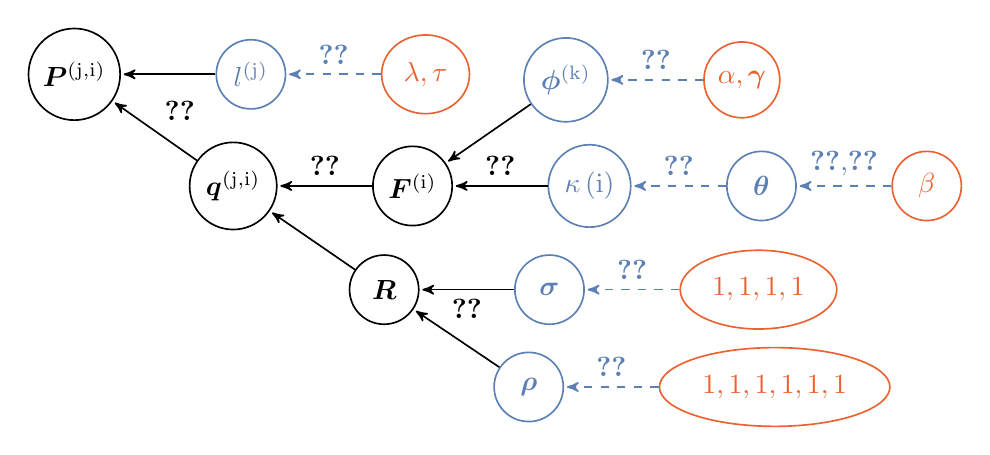
\begin{tikzpicture}[->,>=stealth',shorten >=1pt,auto,node distance=0.6cm and 1.2cm,semithick]
            \tikzstyle{every state}=[]

            \node[state] (P) {$\Probmatrix\branchsiteexp$};
            \node[state] (Q) [below right=of P] {$\Submatrix\branchsiteexp$};
            \node[state] (R) [below right=of Q] {$\Mutmatrix$};
            \node[state] (BL) [BLUE, right=of P] {$\branchlength\branchexp$};
            \node[res] (BLH) [RED, right=of BL] {$ \lambda, \tau $};
            \node[state] (f) [right=of Q] {$\Fit\siteexp $};
            \node[state] (Ex) [BLUE, below right=of R] {$\Exchan$};
            \node[state] (Equi) [BLUE, right=of R] {$\Mutequi$};
            \node[state] (Base) [BLUE, above right=of f] {$\Profile\catexp$};
            \node[state] (cat) [BLUE, right=of f] {$\catsite$};
            \node[res] (ExH) [RED, right=of Ex] {$1,1,1,1,1,1$};
            \node[res] (EquiH) [RED, right=of Equi] {$1,1,1,1$};
            \node[state] (baseH) [RED, right=of Base] {$\concentrationProfile, \centerProfile $};
            \node[state] (sb) [BLUE, right=of cat] {$\StickBreaking$};
            \node[state] (sbH) [RED, right=of sb] {$\stickbreakinghyper$};

            \path
            (Q) edge [black] node [above right] {\ref{eq:Probmatrix}} (P)
            (BL) edge [black] node [] {} (P)
            (R) edge [black] node {} (Q)
            (f) edge [black] node [above] {\ref{eq:subrates}} (Q)
            (Ex) edge [black] node [] {} (R)
            (Equi) edge [black] node [below] {\ref{eq:gtr-mutrates}} (R)
            (Base) edge [black] node {} (f)
            (cat) edge [black] node [above] {\ref{eq:sitefitness}} (f)
            (BLH) edge [dashed, BLUE] node [above] {\ref{eq:branchlength}} (BL)
            (ExH) edge [dashed, BLUE] node [above] {\ref{eq:DistribExchan}} (Ex)
            (EquiH) edge [dashed, BLUE] node [above] {\ref{eq:DistribMutequi}} (Equi)
            (baseH) edge [dashed, BLUE] node [above] {\ref{eq:DistribBase}} (Base)
            (sb) edge [dashed, BLUE] node [above] {\ref{eq:DistribMultinomial}} (cat)
            (sbH) edge [dashed, BLUE] node [above] {\ref{eq:DistribStickBreaking},\ref{eq:Beta}} (sb);
        \end{tikzpicture}
        \captionof{figure}[Bayesian hierarchical model.]{
    \textbf{Bayesian hierarchical model.} Nodes of the directed acyclic graph are the variables, and edges are the functions.
    Hyper-parameters are depicted in {\color{RED}{red}} circles, random variables in {\color{BLUE}{blue}} circles, and transformed variables in black.
    {\color{BLUE}{Blue}} dashed line denotes a drawing from a random distribution, and black solid lines denote a function.
    All the nodes pointing toward a given node (upstream) are its dependencies which determine its distribution.
    The other way around, following the arrows in the DAG (downstream), simple {prior} distributions are combined together to form more complex joint {prior} distributions which ultimately define the {prior} distribution of the model.
    Equations~\ref{eq:gtr-mutrates} to~\ref{eq:Probmatrix} describe the relationship between variables (sections~\ref{sec:nuc} to~\ref{sec:codon}).
    \label{mutsel-illustration}}
    \end{center}



    \subsection{Nucleotide mutation rates}
    \label{sec:nuc}
    The generalized time-reversible (GTR) nucleotide mutation rate matrix $\Mutmatrix$ is a function of the nucleotide frequencies $\Mutequi$ and the symmetric exchangeability rates $\Exchan$~\cite{tavare_probabilistic_1986}.
    $\Mutequi = (\mutequi_A , \mutequi_C , \mutequi_G , \mutequi_T)$ is the equilibrium base frequency vector, giving the frequency at which each base occurs at each site.
    $\Exchan = \left( \exchan_{AC}, \exchan_{AG}, \exchan_{AT}, \exchan_{CG}, \exchan_{CT}, \exchan_{GT}\right)$ is the vector of exchangeabilities between nucleotides.
    Altogether, the rate matrix is:
    \begin{equation}
        \label{eq:gtr-mutrates}
        \Mutmatrix =
        \begin{blockarray}{ccccc}
            & A & C & G & T \\
            \begin{block}{c(cccc)}
                A & -\mu_A & {\exchan_{AC}\mutequi_C} & {\exchan_{AG}\mutequi_G} & {\exchan_{AT}\mutequi_T} \\
                C & {\exchan_{AC}\mutequi_A} &                        -\mu_C & {\exchan_{CG}\mutequi_G} & {\exchan_{CT}\mutequi_T} \\
                G & {\exchan_{AG}\mutequi_A} & {\exchan_{CG}\mutequi_C} &                        -\mu_G & {\exchan_{GT}\mutequi_T} \\
                T & {\exchan_{AT}\mutequi_A} & {\exchan_{CT}\mutequi_C} & {\exchan_{GT}\mutequi_G} & -\mu_T\\
            \end{block}
        \end{blockarray}
    \end{equation}
    By definition, the sum of the entries in each row of the nucleotide rate matrix $\Mutmatrix$ is equal to $0$, giving the diagonal entries:
    \begin{equation}
        \mu_a = \sum\limits_{ b \neq a, b \in \{A, C, G, T\} } \mutmatrix_{a,b}
    \end{equation}
    The {prior} on the exchangeabilities $\Exchan$ is a uniform Dirichlet distribution of dimension $6$:
    \begin{equation}
        \label{eq:DistribExchan}
        \Exchan \sim \text{Dir}\left( 1,1,1,1,1,1 \right).
    \end{equation}
    The {prior} on the equilibrium base frequencies $\Mutequi$ is a uniform Dirichlet distribution of dimension $4$:
    \begin{equation}
        \label{eq:DistribMutequi}
        \Mutequi \sim \text{Dir}\left( 1,1,1,1 \right)
    \end{equation}
    The general time-reversible nucleotide matrix is normalized with a total flow of $1$:
    \begin{equation}
        \sum\limits_{a \in \{A, C, G, T\}} - \mutequi_a \mutmatrix_{a,a} = 1,
    \end{equation}
    such that we expect $1$ {substitution} per unit of branch length.

    \subsection{Site-specific amino-acid fitness profiles}
    \label{sec:profiles}
    Site-specific amino-acid fitness profiles are assumed i.i.d. from a mixture model, itself endowed with a truncated Dirichlet process prior.
    Specifically, the mixture has $\Ncat$ components ($\Ncat = 30$ by default).
    The prior on component weights~($\StickBreaking$) is modeled using a stick-breaking process, truncated at $\Ncat$ and of parameter $\stickbreakinghyper=1$:
    \begin{align}
        \label{eq:DistribStickBreaking}
        \begin{split}
            & \StickBreaking \sim \text{StickBreaking}\left( \Ncat, \stickbreakinghyper \right)\\
            \iff & \stickbreaking_{\cat} = \stick_{\cat}\cdot \prod _{{\indice=1}}^{{\cat-1}}\left(1-\stick_{\indice}\right),\ \Setcat,
        \end{split}
    \end{align}
    where $\stick_{\cat}$ are i.i.d. from a beta distribution
    \begin{equation}
        \label{eq:Beta}
        \stick_{\cat} \sim \text{Beta}\left( 1, \stickbreakinghyper \right),\ \Setcat.
    \end{equation}
    Of note, the weights decrease geometrically in expectation, at rate $\stickbreakinghyper$, such that lower values of $\stickbreakinghyper$ induce more heterogeneous distributions of weights.

    Each component of the mixture defines a 20-dimensional fitness profile $\Profile\catexp$ (summing to $1$), for $ \Setcat$.
    These fitness profiles are i.i.d. from a Dirichlet of center $\centerProfile=1$ and concentration $\concentrationProfile=1$:
    \begin{equation}
        \label{eq:DistribBase}
        \Profile\catexp \sim \text{Dir}\left( \centerProfile,\ \concentrationProfile \right),\ \Setcat.
    \end{equation}

    Site allocations to the mixture components $\catsite \in \catInterval $, for $\Setsite$ running over the $\Nsite$ sites of the alignment, are i.i.d. multinomial of parameter $\StickBreaking$:
    \begin{align}
        \label{eq:DistribMultinomial}
        \catMultiVar \sim \text{Multinomial}\left( \StickBreaking \right), \\
        \text{ where } \catmultivar_{\cat} = \sum_{\Setsite} \mathbb{1}_{\catsite = \cat}
    \end{align}

    For a given parameter configuration for the mixture, the scaled fitness $\Fit\siteexp$ at site $\site$, are obtained by taking the logarithm of fitness assigned to this site:
    \begin{equation}
        \label{eq:sitefitness}
        \Fit\siteexp = \ln \left( \Profile^{\left( \catsite \right)} \right),\ \Setsite.
    \end{equation}

    \subsection{Branch length}
    The topology of the rooted phylogenetic tree is supposed to be known and is not estimated by the model.
    The branch lengths $\branchlength\branchexp$ are defined as the expected number of {neutral} substitutions per {DNA} site along a branch, each from a Gamma distribution of mean $\lambda=0.1$ and scale $\tau=1$:
    \begin{equation}
        \label{eq:branchlength}
        \branchlength\branchexp \sim \text{Gamma}\left( \lambda, \tau \right).
    \end{equation}

    \subsection{Codon substitution rates}
    \label{sec:codon}
    The mutation rate between codons $\ci$ and $\cj$, denoted $\mu_{\itoj}$ depends on the underlying nucleotide change between the codons.
    First, if codons $\ci$ and $\cj$ are not nearest-neighbours, $\mu_{\itoj}$ is equal to $0$.
    Second, if codons $\ci$ and $\cj$ are only one mutation away, $\mu_{\itoj}$ is given by the underlying nucleotide relative rate~(${\mutmatrix_{\itoj}}$).

    For a given site $\site$, the {codon} {substitution} rate matrix $\Submatrix\siteexp$ is given by:
    \begin{equation}
        \label{eq:subrates}
        \begin{dcases}
            \submatrix\siteexp_{\itoj} = 0\text{ if codons $\ci$ and $\cj$ are not nearest-neighbors,} \\
            \submatrix\siteexp_{\itoj} = \mu_{\itoj}\text{ if codons $\ci$ and $\cj$ are {synonymous},} \\
            \submatrix\siteexp_{\itoj} = \mu_{\itoj} \dfrac{ \fitj\siteexp - \fiti\siteexp}{{1 - \e^{\fiti\siteexp - \fitj\siteexp} }} \text{ if codons $\ci$ and $\cj$ are non-synonymous,}\\
            \submatrix\siteexp_{\ci, \ci} = - \sum\limits_{ \cj \neq \ci, \cj=1}^{61} \submatrix\siteexp_{\itoj}.
        \end{dcases}
    \end{equation}
    Together, the probability of transition between codons for a given branch $\branch$ and site $\site$ is:
    \begin{equation}
        \label{eq:Probmatrix}
        \Probmatrix\branchsiteexp = \e^{\branchlength\branchexp \Submatrix\siteexp},
    \end{equation}
    which are the matrices necessary to compute the {likelihood} of the data ($\data$) given the parameters of the model using the pruning algorithm.

    \subsection{Bayesian implementation}
    \label{sec:Bayesian}
    Bayesian inference was conducted using Markov Chain Monte Carlo (MCMC).
    Most phylogenetic {MCMC} samplers target the distribution over the model parameters given the sequence alignment, which means that they have to repeatedly invoke the pruning algorithm to recalculate the {likelihood} which is most often the limiting step of the {MCMC}.
    An alternative, which is used here, is to do the {MCMC} conditionally on the detailed {substitution} history $\subhistory$, thus doing the {MCMC} over the augmented configuration~($\subhistory$, $\data$), under the target distribution obtained by combining the mapping-based {likelihood} with the {prior} over model parameters.
    The key idea that makes this strategy efficient is that the mapping-based {likelihood} depends on compact summary statistics of $\subhistory$, leading to a very fast evaluation of the {likelihood}.
    On the other hand, this requires to implement more complex {MCMC} procedures that have to alternate between:
    \begin{enumerate}
        \item sampling $\subhistory$ conditionally on the data and the current parameter configuration.
        \item re-sampling the parameters conditionally on $\subhistory$.
    \end{enumerate}

    To implement the mapping-based {MCMC} sampling strategy, we first sample the detailed {substitution} history $\subhistory$ for all sites along the tree.
    Several methods exist for doing this~\cite{nielsen_mapping_2002,rodrigue_uniformization_2008}, which are used here in combination: first trying the accept-reject method of \textcite{nielsen_mapping_2002}, then switching to the uniformization approach of \textcite{rodrigue_uniformization_2008} if the first round has failed.

    Then, we write down the probability of $\subhistory$ given the parameters, and finally, we collect all factors that depend on some parameter of interest and make some simplifications.
    This ultimately leads to relatively compact sufficient statistics allowing for fast numerical evaluation of the likelihood~\cite{irvahn_phylogenetic_2014,davydov_state_2017}.

    \subsection{BayesCode software}\label{subsec:bayescode}
    In \textit{BayesCode} (\href{https://github.com/ThibaultLatrille/BayesCode}{github.com/ThibaultLatrille/BayesCode}, v1.3.1), we ran the mutation-selection codon models \textit{mutselomega} for 2000 points of MCMC with the options:
    \begin{scriptsize}
        \begin{verbatim}
 mutselomega ---omegashift 0.0 --ncat 30 -a my_alignment.phy -t my_tree.newick -u 2000 my_genename
        \end{verbatim}
    \end{scriptsize}
    The collection of site-specific fitness profiles ($\UniDimArray{F^{(i)}}, \forall i$) are then obtained by running \textit{readmutselomega}, reading 1000 points of MCMC (first 1000 are considered as burn-in) with the options:
    \begin{scriptsize}
        \begin{verbatim}
 readmutselomega --every 1 --until 2000 --burnin 1000 --ss my_genename
        \end{verbatim}
    \end{scriptsize}
    The gene-specific $4 \times 4$ nucleotide mutation rate matrix ($\UniDimArray{\mu}$) is also obtained by running \textit{readmutselomega}, reading 1000 points of MCMC (first 1000 are considered as burn-in) with the options:
    \begin{scriptsize}
        \begin{verbatim}
 readmutselomega --every 1 --until 2000 --burnin 1000 --nuc my_genename
        \end{verbatim}
    \end{scriptsize}


    \section{Beneficial mutations in the terminal lineages and populations}\label{sec:beneficial-mutations}

    \subsection{Example sites}\label{subsec:example-sites}

    We extracted protein-coding DNA alignments across mammals centered around the codon site (two flanking codons in white background) for which the beneficial non-adaptive mutations ($\SphyBen$) have been detected in \textit{Chlorocebus sabaeus}.
    We also show the translated amino acids of this region.
    For instance, in DNA alignment of gene SELE (\ref{fig:example-1}), the nucleotide at site 1722 has mutated (from T to C) at the basis of Simiiformes (monkeys and apes), modifying the corresponding amino acid from Serine to Proline, but has been subsequently reverted in the branch of \textit{Chlorocebus sabaeus}.
    However, other substitutions classified as $\SphyBen$ cannot be clearly interpreted as reversions \textit{sensu stricto} along the terminal branch of \textit{Chlorocebus sabaeus}.
    Indeed, we acknowledge that on a fixed fitness landscape, a deleterious mutation can be compensated by transitions to other fitter amino-acids, and not necessarily the ancestral one.

    Finally, we generated the fasta alignment for all $\SphyBen$ mutations that we detected, either in the terminal lineage or in segregating polymorphisms.
    These fasta files are available at Zenodo (\url{https://doi.org/10.5281/zenodo.7878953}), across all populations, under a zip file (\textit{alignment\_around\_non\_adaptive\_mutations.zip}) alongside a python script to obtain the figures (as in Figures~\ref{fig:example-1} and~\ref{fig:example-2}) given these alignments (\textit{plot\_variations.py}).

    \newpage
    \begin{center}
        \includegraphics[width=0.9\linewidth, page=1]{artworks/Alignment.Chlorocebus_sabaeus.Saint_Kitts-0.pdf}
        \captionof{figure}[Examples sites of $\SphyBen$ mutations in \textit{Chlorocebus sabaeus} (reversions).]{\textbf{Examples sites of $\bm{\SphyBen}$ mutations in \textit{Chlorocebus sabaeus}  (reversions).} The first line is the name of the gene, the second line the position of the mutation in the OrthoMam protein-coding DNA alignment, and the arrows in the third line correspond to the position of the mutation in the nucleotide sequence (left) and in the corresponding amino acid sequence (right)\label{fig:example-1}}
    \end{center}

    \newpage
    \begin{center}
        \includegraphics[width=0.9\linewidth, page=1]{artworks/Alignment.Chlorocebus_sabaeus.Saint_Kitts-1.pdf}
        \captionof{figure}[Examples sites of $\SphyBen$ mutations in \textit{Chlorocebus sabaeus}.]{\textbf{Examples sites of $\bm{\SphyBen}$ mutations in \textit{Chlorocebus sabaeus}.} The first line is the name of the gene, the second line the position of the mutation in the OrthoMam protein-coding DNA alignment, and the arrows in the third line correspond to the position of the mutation in the nucleotide sequence (left) and in the corresponding amino acid sequence (right).\label{fig:example-2}}
    \end{center}

    \newpage
    \subsection{Selection along the terminal branches}\label{subsec:summary-table-mutsel}

    \subsubsection{Probability of mutations and substitutions to be \texorpdfstring{$\SphyDel$}{D₀}, \texorpdfstring{$\SphyNeu$}{N₀} or \texorpdfstring{$\SphyBen$}{B₀}}
    Among all the substitutions found in each terminal branch, between 10 and 13\% were $\SphyBen$ ($\proba_{div}[ \SphyBen {]}$), while $\SphyBen$ mutations only represent between 0.9 and 1.2\% of all non-synonymous mutations ($\proba[ \SphyBen {]}$), as shown in Table~\ref{table:pdiv}.

    \begin{center}
        \scriptsize
        \begin{longtable*}{|l|l|r|r|r|r|r|r|}
            \toprule
            Population &             Species & $\proba{[} \SphyDel {]}$ & $\proba{[} \SphyNeu {]}$ & $\proba{[} \SphyBen {]}$ & $\proba_{div}[ \SphyDel {]}$ & $\proba_{div}[ \SphyNeu {]}$ & $\proba_{div}[ \SphyBen {]}$ \\
            \midrule
            \endhead
            \midrule
            \multicolumn{8}{r}{{Continued on next page}} \\
            \midrule
            \endfoot

            \bottomrule
            \endlastfoot
            \rowcolor{LIGHTGREY} Equus c. & Equus caballus & $ 0.923$ & $ 0.065$ & $ 0.012$ & $ 0.462$ & $ 0.419$ & $ 0.118$ \\
            Iran & Bos taurus & $ 0.924$ & $ 0.065$ & $ 0.011$ & $ 0.515$ & $ 0.362$ & $ 0.123$ \\
            Uganda & Bos taurus & $ 0.924$ & $ 0.065$ & $ 0.011$ & $ 0.514$ & $ 0.361$ & $ 0.125$ \\
            \rowcolor{LIGHTGREY} Australia & Capra hircus & $ 0.923$ & $ 0.066$ & $ 0.011$ & $ 0.494$ & $ 0.386$ & $ 0.121$ \\
            \rowcolor{LIGHTGREY} France & Capra hircus & $ 0.923$ & $ 0.066$ & $ 0.011$ & $ 0.494$ & $ 0.386$ & $ 0.120$ \\
            \rowcolor{LIGHTGREY} Iran (C. aegagrus) & Capra hircus & $ 0.923$ & $ 0.066$ & $ 0.011$ & $ 0.493$ & $ 0.386$ & $ 0.120$ \\
            \rowcolor{LIGHTGREY} Iran & Capra hircus & $ 0.923$ & $ 0.066$ & $ 0.011$ & $ 0.492$ & $ 0.387$ & $ 0.121$ \\
            \rowcolor{LIGHTGREY} Italy & Capra hircus & $ 0.923$ & $ 0.066$ & $ 0.011$ & $ 0.494$ & $ 0.386$ & $ 0.120$ \\
            \rowcolor{LIGHTGREY} Morocco & Capra hircus & $ 0.923$ & $ 0.066$ & $ 0.011$ & $ 0.491$ & $ 0.387$ & $ 0.122$ \\
            Iran & Ovis aries & $ 0.922$ & $ 0.067$ & $ 0.012$ & $ 0.568$ & $ 0.323$ & $ 0.109$ \\
            Iran (O. orientalis) & Ovis aries & $ 0.922$ & $ 0.067$ & $ 0.011$ & $ 0.573$ & $ 0.320$ & $ 0.108$ \\
            Iran (O. vignei) & Ovis aries & $ 0.922$ & $ 0.067$ & $ 0.012$ & $ 0.567$ & $ 0.325$ & $ 0.109$ \\
            Various & Ovis aries & $ 0.922$ & $ 0.067$ & $ 0.011$ & $ 0.572$ & $ 0.321$ & $ 0.107$ \\
            Morocco & Ovis aries & $ 0.922$ & $ 0.067$ & $ 0.012$ & $ 0.570$ & $ 0.321$ & $ 0.108$ \\
            \rowcolor{LIGHTGREY} Barbados & Chlorocebus sabaeus & $ 0.926$ & $ 0.065$ & $ 0.009$ & $ 0.485$ & $ 0.393$ & $ 0.122$ \\
            \rowcolor{LIGHTGREY} Central Afr. Rep. & Chlorocebus sabaeus & $ 0.926$ & $ 0.065$ & $ 0.009$ & $ 0.485$ & $ 0.391$ & $ 0.124$ \\
            \rowcolor{LIGHTGREY} Ethiopia & Chlorocebus sabaeus & $ 0.926$ & $ 0.065$ & $ 0.009$ & $ 0.484$ & $ 0.393$ & $ 0.124$ \\
            \rowcolor{LIGHTGREY} Gambia & Chlorocebus sabaeus & $ 0.926$ & $ 0.065$ & $ 0.009$ & $ 0.483$ & $ 0.394$ & $ 0.123$ \\
            \rowcolor{LIGHTGREY} Kenya & Chlorocebus sabaeus & $ 0.926$ & $ 0.065$ & $ 0.009$ & $ 0.485$ & $ 0.392$ & $ 0.123$ \\
            \rowcolor{LIGHTGREY} Nevis & Chlorocebus sabaeus & $ 0.926$ & $ 0.065$ & $ 0.009$ & $ 0.484$ & $ 0.393$ & $ 0.123$ \\
            \rowcolor{LIGHTGREY} South Africa & Chlorocebus sabaeus & $ 0.926$ & $ 0.065$ & $ 0.009$ & $ 0.480$ & $ 0.394$ & $ 0.125$ \\
            \rowcolor{LIGHTGREY} Saint Kitts & Chlorocebus sabaeus & $ 0.926$ & $ 0.065$ & $ 0.009$ & $ 0.483$ & $ 0.394$ & $ 0.123$ \\
            \rowcolor{LIGHTGREY} Zambia & Chlorocebus sabaeus & $ 0.926$ & $ 0.065$ & $ 0.009$ & $ 0.485$ & $ 0.393$ & $ 0.123$ \\
            African & Homo sapiens & $ 0.925$ & $ 0.065$ & $ 0.010$ & $ 0.561$ & $ 0.341$ & $ 0.099$ \\
            Admixed American & Homo sapiens & $ 0.925$ & $ 0.065$ & $ 0.010$ & $ 0.561$ & $ 0.340$ & $ 0.099$ \\
            East Asian & Homo sapiens & $ 0.925$ & $ 0.065$ & $ 0.010$ & $ 0.560$ & $ 0.341$ & $ 0.098$ \\
            European & Homo sapiens & $ 0.925$ & $ 0.065$ & $ 0.010$ & $ 0.562$ & $ 0.340$ & $ 0.098$ \\
            South Asian & Homo sapiens & $ 0.925$ & $ 0.065$ & $ 0.010$ & $ 0.561$ & $ 0.341$ & $ 0.099$ \\
        \end{longtable*}
    \captionof{table}[Probability of mutations and substitutions to be $\SphyDel$, $\SphyNeu$ or $\SphyBen$.]{\textbf{Probability of mutations and substitutions to be $\bm{\SphyDel}$, $\bm{\SphyNeu}$ or $\bm{\SphyBen}$.}
    $\proba{[} \SphyDel {]}$ (eq.~5) is the probability for a new mutation to be deleterious.
     These mutations have a selection coefficient predicted at the phylogenetic-scale lower than -1, thus toward a less fit amino-acid.
    $\proba{[} \SphyNeu {]}$ (eq.~5) is the probability for a new mutation to be nearly-neutral.
    These mutations have a selection coefficient predicted at the phylogenetic-scale between -1 and 1.
    $\proba{[} \SphyBen {]}$ (eq.~5) is the probability for a new mutation to be non-adaptive beneficial.
    These mutations have a selection coefficient predicted at the phylogenetic-scale larger than 1, thus toward a more fit amino-acid.
    $\proba_{div}[\SphyDel{]}$ is the proportion of substitutions in the terminal branch that are $\SphyDel$.
    $\proba_{div}[\SphyNeu{]}$ is the proportion of substitutions in the terminal branch that are $\SphyNeu$.
    $\proba_{div}[\SphyBen{]}$ is the proportion of substitutions in the terminal branch that are $\SphyBen$.\label{table:pdiv}}
    \end{center}
    \newpage

    \subsubsection{\texorpdfstring{$\dnds$}{dₙ/dₛ} for \texorpdfstring{$\SphyDel$}{D₀}, \texorpdfstring{$\SphyNeu$}{N₀} or \texorpdfstring{$\SphyBen$}{B₀}}
    Theoretically, $\omega = \dn / \ds$ can be related to the underlying scaled selection coefficient ($S$) with the relation $\omega = S /(1-\exp(-S))$ as in \cite[eq. 3]{nielsen_estimating_2003}.
    In our experiments, our observed $\dn(\SphyBen) / \ds$ is within the range of $1.169$ (\textit{C. hircus}) to 1.745 (\textit{H. sapiens}), as shown in Table~\ref{table:dnds}, translating into an average $S$ of $\approx0.32$ to $\approx1.24$, so indeed only slightly advantageous.\\

    Of note, observing $\dn(\SphyBen) / \ds >1$ is an important check that $\SphyBen$ mutations are indeed positively selected with an increased substitution rate.
    Since $\dn(\SphyNeu) / \ds$ is close to 1 for the predicted nearly-neutral mutations, this means that the selection coefficients predicted at the mutation-selection balance are good proxies of selection, then observing $\dn(\SphyBen) / \ds > 1$ is evidence of positive selection of predicted non-adaptive beneficial mutations.
    \begin{center}
        \scriptsize
        \begin{longtable*}{|l|r|r|r|r|}
            \toprule
            Species & $\dnds $ & $\dn ( \SphyDel ) / \ds$ & $\dn ( \SphyNeu ) / \ds$ & $\dn ( \SphyBen ) / \ds$ \\
            \midrule
            \endhead
            \midrule
            \multicolumn{5}{r}{{Continued on next page}} \\
            \midrule
            \endfoot

            \bottomrule
            \endlastfoot
            \rowcolor{LIGHTGREY} Equus caballus & $ 0.129$ & $ 0.065$ & $ 0.832$ & $ 1.267$ \\
            Bos taurus & [$ 0.114$, $ 0.116$] & [$ 0.063$, $ 0.064$] & [$ 0.629$, $ 0.638$] & [$ 1.280$, $ 1.328$] \\
            \rowcolor{LIGHTGREY} Capra hircus & [$ 0.108$, $ 0.109$] & [$ 0.058$, $ 0.058$] & [$ 0.631$, $ 0.636$] & [$ 1.169$, $ 1.183$] \\
            Ovis aries & [$ 0.127$, $ 0.129$] & [$ 0.078$, $ 0.080$] & [$ 0.619$, $ 0.621$] & [$ 1.201$, $ 1.217$] \\
            \rowcolor{LIGHTGREY} Chlorocebus sabaeus & [$ 0.118$, $ 0.119$] & [$ 0.062$, $ 0.062$] & [$ 0.713$, $ 0.720$] & [$ 1.521$, $ 1.577$] \\
            Homo sapiens & [$ 0.170$, $ 0.170$] & [$ 0.103$, $ 0.103$] & [$ 0.884$, $ 0.888$] & [$ 1.733$, $ 1.745$] \\
        \end{longtable*}
    \captionof{table}[$\dnds$ for $\SphyDel$, $\SphyNeu$ or $\SphyBen$.]{\textbf{$\bm{\dnds}$ for $\bm{\SphyDel}$, $\bm{\SphyNeu}$ or $\bm{\SphyBen}$.}
    $\dnds$ (eq.~6) is the ratio of non-synonymous over synonymous substitutions estimated for all the non-synonymous substitutions in the terminal branch.
    $\dn(\SphyDel) / \ds$ (eq.~6) is the ratio of non-synonymous over synonymous substitutions, when restricted to non-synonymous substitutions in the terminal branch that are $\SphyDel$.
    $\dn(\SphyNeu) / \ds$ (eq.~6) is the ratio of non-synonymous over synonymous substitutions, when restricted to non-synonymous substitutions in the terminal branch that are $\SphyNeu$.
    $\dn(\SphyBen) / \ds$ (eq.~6) is the ratio of non-synonymous over synonymous substitutions, when restricted to non-synonymous substitutions in the terminal branch that are $\SphyBen$.
    SNPs are considered fixed (as a substitution) in the populations if all sampled individuals are homozygous for the derived allele.
    This effect results in $\dn / \ds$ varying across populations, denoted as a range per species.
    $\dn(\SphyBen) / \ds$ values observed are above 1 and are consistent with slightly advantageous mutations.\label{table:dnds}}
    \end{center}


    \newpage
    \subsubsection{\texorpdfstring{$\dnds$}{dₙ/dₛ} over-estimation due to non-adaptive beneficial mutations}
    We estimated that between $\approx9$ and $\approx12\%$ of $\dnds$ is over-estimated, corresponding to non-adaptive beneficial mutations inflating the $\dnds$ statistic, as shown in Table~\ref{table:dnds-delta}.
    \begin{center}
        \scriptsize
        \begin{longtable*}{|l|r|r|r|}
            \toprule
            Species & $\dnds $ & $\dn(\Sphy < 1) / \ds$ & $\delta(\dnds )$ \\
            \midrule
            \endhead
            \midrule
            \multicolumn{4}{r}{{Continued on next page}} \\
            \midrule
            \endfoot

            \bottomrule
            \endlastfoot
            \rowcolor{LIGHTGREY} Equus caballus & $ 0.129$ & $ 0.115$ & $  10.7$ \\
            Bos taurus & [$ 0.114$, $ 0.116$] & [$ 0.101$, $ 0.102$] & [$  11.3$, $  11.5$] \\
            \rowcolor{LIGHTGREY} Capra hircus & [$ 0.108$, $ 0.109$] & [$ 0.096$, $ 0.097$] & [$  11.0$, $  11.2$] \\
            Chlorocebus sabaeus & [$ 0.118$, $ 0.119$] & [$ 0.104$, $ 0.105$] & [$  11.4$, $  11.7$] \\
            \rowcolor{LIGHTGREY} Homo sapiens & [$ 0.170$, $ 0.170$] & [$ 0.154$, $ 0.155$] & [$ 8.926$, $ 8.996$] \\
            Ovis aries & [$ 0.127$, $ 0.129$] & [$ 0.115$, $ 0.117$] & [$ 9.663$, $ 9.894$] \\
        \end{longtable*}
        \captionof{table}[$\dnds$ over-estimation due to non-adaptive beneficial mutations.]{\textbf{$\bm{\dnds}$ over-estimation due to non-adaptive beneficial mutations.}
        $\dnds$ (eq.~6) is the ratio of non-synonymous over synonymous substitutions estimated for all the non-synonymous substitutions in the terminal branch.
        $\dn(\Sphy < 1) / \ds$ (eq.~6) is the ratio of non-synonymous over synonymous substitutions, when restricted to non-synonymous substitutions in the terminal branch that are not $\SphyBen$.
        This is the estimated divergence when we remove non-adaptive beneficial mutations.
        $\delta(\dnds)$ (eq.~7) is the fraction of the divergence ($\dnds$) that is over-estimated: the difference between $\dnds$ and $\dn(\Sphy < 1) / \ds$.\label{table:dnds-delta}}
    \end{center}
    \newpage
    \section{Gene ontology enrichment}

    \subsection{Gene ontology enrichment in \texorpdfstring{$\SphyBen$}{B₀} SNPs}

    To assess whether $\SphyBen$ SNPs are enriched in specific gene functions, we used gene ontology (GO) terms at the gene level.
    Thus, for each $\SphyBen$ SNP detected in a focal population, we annotated this SNP with GO terms inherited from the gene in which the SNP is located.
    We restricted this analysis solely on genes annotated with at least one GO term.
    To assess the weight of each GO term in the set of $\SphyBen$ SNPs, we computed the proportion of $\SphyBen$ SNPs annotated with a given GO term.
    We then tested if the distribution of $\SphyBen$ SNPs is different between genes sharing a common GO term and the rest of the genes, as shown in Table~\ref{table:ontology}.

    \begin{center}
        \scriptsize
        \begin{longtable*}{|l|l|r|r|r|r|r|}
            \toprule
            GO id & GO name & $p$ & $r$ & Mann-Whitney U & $p_{\mathrm{v}}$ & $p_{\mathrm{v}}^{\mathrm{adj}}$ \\
            \midrule
            \endhead
            \midrule
            \multicolumn{7}{r}{Continued on next page} \\
            \midrule
            \endfoot
            \bottomrule
            \endlastfoot
            GO:0003777 & microtubule motor activity & $ 0.027$ & $ 1.802$ & $1.1\times 10^{5}$ & $1.8\times 10^{-6}$ & $\bm{0.0008{^*}}$ \\
            GO:0005578 & proteinaceous extracellular matrix & $ 0.069$ & $ 2.071$ & $4.7\times 10^{5}$ & $1.9\times 10^{-6}$ & $\bm{0.00084{^*}}$ \\
            GO:0003774 & motor activity & $ 0.023$ & $ 1.127$ & $1.1\times 10^{5}$ & $6.7\times 10^{-5}$ & $\bm{ 0.029{^*}}$ \\
            GO:0030198 & extracellular matrix organization & $ 0.039$ & $ 1.956$ & $2.7\times 10^{5}$ & $0.00055$ & $ 0.239~~$ \\
            GO:0007018 & microtubule-based movement & $ 0.023$ & $ 0.924$ & $1.3\times 10^{5}$ & $0.00073$ & $ 0.315~~$ \\
            GO:0005576 & extracellular region & $ 0.178$ & $ 2.195$ & $1.9\times 10^{6}$ & $0.00083$ & $ 0.359~~$ \\
            GO:0006898 & receptor-mediated endocytosis & $ 0.027$ & $ 1.803$ & $1.7\times 10^{5}$ & $ 0.001$ & $ 0.512~~$ \\
            GO:0006355 & regulation of transcription & $ 0.069$ & $ 0.275$ & $1.9\times 10^{6}$ & $ 0.002$ & $ 0.815~~$ \\
            GO:0005604 & basement membrane & $ 0.019$ & $ 1.638$ & $1.1\times 10^{5}$ & $ 0.002$ & $ 0.852~~$ \\
            GO:0007229 & integrin-mediated signaling pathway & $ 0.019$ & $ 1.930$ & $1.1\times 10^{5}$ & $ 0.003$ & $ 1.000~~$ \\
            GO:0016887 & ATPase activity & $ 0.031$ & $ 1.149$ & $1.8\times 10^{5}$ & $ 0.003$ & $ 1.000~~$ \\
            GO:0007155 & cell adhesion & $ 0.062$ & $ 1.438$ & $5.8\times 10^{5}$ & $ 0.005$ & $ 1.000~~$ \\
            GO:0005634 & nucleus & $ 0.266$ & $ 0.557$ & $3.9\times 10^{6}$ & $ 0.005$ & $ 1.000~~$ \\
            GO:0006351 & transcription & $ 0.073$ & $ 0.339$ & $1.9\times 10^{6}$ & $ 0.008$ & $ 1.000~~$ \\
            GO:0005654 & nucleoplasm & $ 0.124$ & $ 0.443$ & $2.6\times 10^{6}$ & $ 0.009$ & $ 1.000~~$ \\
            GO:0006366 & transcription from RNA polymerase II promoter & $ 0.008$ & $ 0.063$ & $6.2\times 10^{5}$ & $ 0.011$ & $ 1.000~~$ \\
            GO:0005829 & cytosol & $ 0.212$ & $ 0.541$ & $3.5\times 10^{6}$ & $ 0.012$ & $ 1.000~~$ \\
            GO:0016853 & isomerase activity & $ 0.015$ & $ 4.066$ & $ 1\times 10^{5}$ & $ 0.015$ & $ 1.000~~$ \\
            GO:0071356 & cellular response to tumor necrosis factor & $ 0.015$ & $ 7.069$ & $ 1\times 10^{5}$ & $ 0.016$ & $ 1.000~~$ \\
            GO:0005518 & collagen binding & $ 0.015$ & $ 2.900$ & $ 1\times 10^{5}$ & $ 0.017$ & $ 1.000~~$ \\
            GO:0043087 & regulation of GTPase activity & $ 0.015$ & $ 2.025$ & $1.1\times 10^{5}$ & $ 0.027$ & $ 1.000~~$ \\
            GO:0000139 & Golgi membrane & $ 0.012$ & $ 0.214$ & $6.3\times 10^{5}$ & $ 0.028$ & $ 1.000~~$ \\
            GO:0043235 & receptor complex & $ 0.023$ & $ 0.935$ & $1.9\times 10^{5}$ & $ 0.028$ & $ 1.000~~$ \\
            GO:0000981 & RNA polymerase II transcription factor activity & $ 0.027$ & $ 0.452$ & $9.1\times 10^{5}$ & $ 0.029$ & $ 1.000~~$ \\
            GO:0005739 & mitochondrion & $ 0.058$ & $ 0.471$ & $1.4\times 10^{6}$ & $ 0.029$ & $ 1.000~~$ \\
            GO:0005581 & collagen trimer & $ 0.015$ & $ 2.124$ & $1.1\times 10^{5}$ & $ 0.036$ & $ 1.000~~$ \\
            GO:0051015 & actin filament binding & $ 0.019$ & $ 0.912$ & $1.5\times 10^{5}$ & $ 0.036$ & $ 1.000~~$ \\
            GO:0001843 & neural tube closure & $ 0.015$ & $ 1.164$ & $1.1\times 10^{5}$ & $ 0.036$ & $ 1.000~~$ \\
            GO:0005737 & cytoplasm & $ 0.317$ & $ 0.692$ & $4.1\times 10^{6}$ & $ 0.037$ & $ 1.000~~$ \\
            GO:0043565 & sequence-specific DNA binding & $ 0.015$ & $ 0.308$ & $ 6\times 10^{5}$ & $ 0.039$ & $ 1.000~~$ \\
            GO:0004222 & metalloendopeptidase activity & $ 0.019$ & $ 1.188$ & $1.6\times 10^{5}$ & $ 0.043$ & $ 1.000~~$ \\
            GO:0007166 & cell surface receptor signaling pathway & $ 0.031$ & $ 2.871$ & $ 3\times 10^{5}$ & $ 0.046$ & $ 1.000~~$ \\
            GO:0007156 & homophilic cell adhesion via plasma membrane... & $ 0.015$ & $ 1.013$ & $1.2\times 10^{5}$ & $ 0.050$ & $ 1.000~~$ \\
            GO:0007286 & spermatid development & $ 0.015$ & $ 2.497$ & $1.2\times 10^{5}$ & $ 0.051$ & $ 1.000~~$ \\
            GO:0008202 & steroid metabolic process & $ 0.015$ & $ 2.755$ & $1.2\times 10^{5}$ & $ 0.051$ & $ 1.000~~$ \\
            GO:0061024 & membrane organization & $ 0.019$ & $ 1.516$ & $1.6\times 10^{5}$ & $ 0.052$ & $ 1.000~~$ \\
            GO:1901796 & regulation of signal transduction by p53 class... & $ 0.019$ & $ 1.333$ & $1.6\times 10^{5}$ & $ 0.058$ & $ 1.000~~$ \\
            GO:0006397 & mRNA processing & $ 0.004$ & $ 0.210$ & $3.5\times 10^{5}$ & $ 0.061$ & $ 1.000~~$ \\
            GO:0006915 & apoptotic process & $ 0.015$ & $ 0.463$ & $6.4\times 10^{5}$ & $ 0.065$ & $ 1.000~~$ \\
            GO:0043547 & positive regulation of GTPase activity & $ 0.035$ & $ 2.651$ & $3.7\times 10^{5}$ & $ 0.068$ & $ 1.000~~$ \\
            GO:0007010 & cytoskeleton organization & $ 0.019$ & $ 1.771$ & $1.7\times 10^{5}$ & $ 0.068$ & $ 1.000~~$ \\
            GO:0030308 & negative regulation of cell growth & $ 0.015$ & $ 3.055$ & $1.3\times 10^{5}$ & $ 0.070$ & $ 1.000~~$ \\
            GO:0007160 & cell-matrix adhesion & $ 0.015$ & $ 1.046$ & $1.2\times 10^{5}$ & $ 0.073$ & $ 1.000~~$ \\
            GO:0006897 & endocytosis & $ 0.023$ & $ 1.408$ & $2.2\times 10^{5}$ & $ 0.073$ & $ 1.000~~$ \\
            GO:0003677 & DNA binding & $ 0.077$ & $ 0.448$ & $1.7\times 10^{6}$ & $ 0.075$ & $ 1.000~~$ \\
            GO:0043202 & lysosomal lumen & $ 0.015$ & $ 1.522$ & $1.3\times 10^{5}$ & $ 0.075$ & $ 1.000~~$ \\
            GO:0003700 & DNA binding transcription factor activity & $ 0.027$ & $ 0.343$ & $8.7\times 10^{5}$ & $ 0.076$ & $ 1.000~~$ \\
            GO:0008134 & transcription factor binding & $ 0.004$ & $ 0.048$ & $3.2\times 10^{5}$ & $ 0.077$ & $ 1.000~~$ \\
            GO:0005488 & binding & $ 0.046$ & $ 0.641$ & $4.1\times 10^{5}$ & $ 0.078$ & $ 1.000~~$ \\
            GO:0045944 & positive regulation of transcription from RNA... & $ 0.039$ & $ 0.324$ & $1.1\times 10^{6}$ & $ 0.085$ & $ 1.000~~$ \\
            GO:0005794 & Golgi apparatus & $ 0.046$ & $ 0.430$ & $1.2\times 10^{6}$ & $ 0.087$ & $ 1.000~~$ \\
            GO:0016032 & viral process & $ 0.008$ & $ 0.321$ & $4.1\times 10^{5}$ & $ 0.089$ & $ 1.000~~$ \\
            GO:0055085 & transmembrane transport & $ 0.054$ & $ 1.533$ & $5.9\times 10^{5}$ & $ 0.092$ & $ 1.000~~$ \\
            GO:0006260 & DNA replication & $ 0.019$ & $ 1.051$ & $1.8\times 10^{5}$ & $ 0.096$ & $ 1.000~~$ \\
            GO:0030425 & dendrite & $ 0.008$ & $ 0.121$ & $3.9\times 10^{5}$ & $ 0.099$ & $ 1.000~~$ \\
            GO:0005524 & ATP binding & $ 0.127$ & $ 0.666$ & $1.5\times 10^{6}$ & $ 0.103$ & $ 1.000~~$ \\
            GO:0005615 & extracellular space & $ 0.100$ & $ 1.699$ & $1.3\times 10^{6}$ & $ 0.107$ & $ 1.000~~$ \\
            GO:0007283 & spermatogenesis & $ 0.039$ & $ 1.824$ & $3.9\times 10^{5}$ & $ 0.108$ & $ 1.000~~$ \\
            GO:0005179 & hormone activity & $ 0.012$ & $ 7.683$ & $9.9\times 10^{4}$ & $ 0.118$ & $ 1.000~~$ \\
            GO:0098793 & presynapse & $ 0.012$ & $ 2.065$ & $9.6\times 10^{4}$ & $ 0.119$ & $ 1.000~~$ \\
            GO:0005254 & chloride channel activity & $ 0.012$ & $ 1.694$ & $9.6\times 10^{4}$ & $ 0.124$ & $ 1.000~~$ \\
            GO:0036064 & ciliary basal body & $ 0.015$ & $ 1.378$ & $1.4\times 10^{5}$ & $ 0.125$ & $ 1.000~~$ \\
            GO:0070062 & extracellular exosome & $ 0.104$ & $ 0.570$ & $2.1\times 10^{6}$ & $ 0.125$ & $ 1.000~~$ \\
            GO:0090630 & activation of GTPase activity & $ 0.012$ & $ 2.519$ & $9.9\times 10^{4}$ & $ 0.127$ & $ 1.000~~$ \\
            GO:0044212 & transcription regulatory region DNA binding & $ 0.004$ & $ 0.322$ & $2.7\times 10^{5}$ & $ 0.128$ & $ 1.000~~$ \\
            GO:0055114 & oxidation-reduction process & $ 0.019$ & $ 0.482$ & $6.4\times 10^{5}$ & $ 0.129$ & $ 1.000~~$ \\
            GO:0019886 & antigen processing and presentation of exogenous... & $ 0.012$ & $ 1.393$ & $9.6\times 10^{4}$ & $ 0.129$ & $ 1.000~~$ \\
            GO:0005743 & mitochondrial inner membrane & $ 0.008$ & $ 0.463$ & $3.7\times 10^{5}$ & $ 0.133$ & $ 1.000~~$ \\
            GO:0022617 & extracellular matrix disassembly & $ 0.012$ & $ 1.009$ & $9.6\times 10^{4}$ & $ 0.135$ & $ 1.000~~$ \\
            GO:0042493 & response to drug & $ 0.004$ & $ 0.043$ & $2.6\times 10^{5}$ & $ 0.137$ & $ 1.000~~$ \\
            GO:0008380 & RNA splicing & $ 0.008$ & $ 0.098$ & $2.6\times 10^{5}$ & $ 0.139$ & $ 1.000~~$ \\
            GO:0043687 & post-translational protein modification & $ 0.008$ & $ 0.319$ & $3.6\times 10^{5}$ & $ 0.140$ & $ 1.000~~$ \\
            GO:0010951 & negative regulation of endopeptidase activity & $ 0.012$ & $ 2.037$ & $9.9\times 10^{4}$ & $ 0.140$ & $ 1.000~~$ \\
            GO:0000978 & RNA polymerase II proximal promoter... & $ 0.012$ & $ 0.250$ & $4.5\times 10^{5}$ & $ 0.140$ & $ 1.000~~$ \\
            GO:0003713 & transcription coactivator activity & $ 0.004$ & $ 0.339$ & $2.6\times 10^{5}$ & $ 0.142$ & $ 1.000~~$ \\
            GO:0001227 & transcriptional repressor activity & $ 0.012$ & $ 1.384$ & $9.9\times 10^{4}$ & $ 0.144$ & $ 1.000~~$ \\
            GO:0005623 & cell & $ 0.012$ & $ 1.927$ & $ 1\times 10^{5}$ & $ 0.150$ & $ 1.000~~$ \\
            GO:0030574 & collagen catabolic process & $ 0.012$ & $ 1.036$ & $9.9\times 10^{4}$ & $ 0.151$ & $ 1.000~~$ \\
            GO:0006457 & protein folding & $ 0.015$ & $ 2.465$ & $1.5\times 10^{5}$ & $ 0.158$ & $ 1.000~~$ \\
            GO:0016477 & cell migration & $ 0.004$ & $ 0.121$ & $2.4\times 10^{5}$ & $ 0.159$ & $ 1.000~~$ \\
            GO:0070374 & positive regulation of ERK1 and ERK2 cascade & $ 0.019$ & $ 4.238$ & $ 2\times 10^{5}$ & $ 0.160$ & $ 1.000~~$ \\
            GO:0007605 & sensory perception of sound & $ 0.015$ & $ 0.824$ & $1.5\times 10^{5}$ & $ 0.162$ & $ 1.000~~$ \\
            GO:0031225 & anchored component of membrane & $ 0.012$ & $ 0.892$ & $ 1\times 10^{5}$ & $ 0.171$ & $ 1.000~~$ \\
            GO:0016757 & transferase activity & $ 0.004$ & $ 0.435$ & $2.4\times 10^{5}$ & $ 0.177$ & $ 1.000~~$ \\
            GO:0002376 & immune system process & $ 0.012$ & $ 0.411$ & $4.3\times 10^{5}$ & $ 0.177$ & $ 1.000~~$ \\
            GO:0005759 & mitochondrial matrix & $ 0.008$ & $ 0.361$ & $3.3\times 10^{5}$ & $ 0.185$ & $ 1.000~~$ \\
            GO:0010389 & regulation of G2/M transition of mitotic cell... & $ 0.012$ & $ 0.924$ & $ 1\times 10^{5}$ & $ 0.188$ & $ 1.000~~$ \\
            GO:0005667 & transcription factor complex & $ 0.004$ & $ 0.177$ & $2.3\times 10^{5}$ & $ 0.189$ & $ 1.000~~$ \\
            GO:0030054 & cell junction & $ 0.031$ & $ 0.251$ & $8.1\times 10^{5}$ & $ 0.190$ & $ 1.000~~$ \\
            GO:0001650 & fibrillar center & $ 0.019$ & $ 1.540$ & $1.1\times 10^{5}$ & $ 0.191$ & $ 1.000~~$ \\
            GO:0014069 & postsynaptic density & $ 0.004$ & $ 0.172$ & $2.2\times 10^{5}$ & $ 0.200$ & $ 1.000~~$ \\
            GO:0046934 & phosphatidylinositol-4 & $ 0.012$ & $ 1.135$ & $1.1\times 10^{5}$ & $ 0.201$ & $ 1.000~~$ \\
            GO:0007267 & cell-cell signaling & $ 0.004$ & $ 0.354$ & $2.2\times 10^{5}$ & $ 0.201$ & $ 1.000~~$ \\
            GO:0001649 & osteoblast differentiation & $ 0.012$ & $ 1.917$ & $1.1\times 10^{5}$ & $ 0.201$ & $ 1.000~~$ \\
            GO:0045893 & positive regulation of transcription & $ 0.023$ & $ 0.596$ & $6.6\times 10^{5}$ & $ 0.205$ & $ 1.000~~$ \\
            GO:0007399 & nervous system development & $ 0.015$ & $ 0.450$ & $ 5\times 10^{5}$ & $ 0.205$ & $ 1.000~~$ \\
            GO:0001501 & skeletal system development & $ 0.015$ & $ 1.212$ & $1.6\times 10^{5}$ & $ 0.207$ & $ 1.000~~$ \\
            GO:0019903 & protein phosphatase binding & $ 0.012$ & $ 0.875$ & $1.1\times 10^{5}$ & $ 0.208$ & $ 1.000~~$ \\
            GO:1902476 & chloride transmembrane transport & $ 0.012$ & $ 1.458$ & $1.1\times 10^{5}$ & $ 0.210$ & $ 1.000~~$ \\
            GO:0007568 & aging & $ 0.015$ & $ 2.053$ & $1.6\times 10^{5}$ & $ 0.210$ & $ 1.000~~$ \\
        \end{longtable*}
        \captionof{table}[Gene ontology enrichment in $\SphyBen$ SNPs.]{\textbf{Gene ontology enrichment in $\bm{\SphyBen}$ SNPs.} GO terms that are enriched in genes with $\SphyBen$ SNPs in European humans (shown here are the first 100 rows with the lowest $p_{\mathrm{v}}$).
        For each GO term, $p$ is the proportion of $\SphyBen$ SNPs that are annotated with this focal GO term among all annotated $\SphyBen$ SNPs.
        For each gene, $p[ \SphyBen {]}$ is the proportion of sites that have a $\SphyBen$ SNP (can be 0 if no $\SphyBen$ SNP is detected for this gene).
        For each GO term, $r$ is the ratio of the mean of $p[ \SphyBen {]}$ in the set of genes sharing the focal ontology over the mean of $p[ \SphyBen {]}$ in the rest of the genes.
        Mann-Whitney U is the statistic testing if the distribution of $p[ \SphyBen {]}$ is different between the two sets of genes (p-value $p_{\mathrm{v}}$ for the two-sided test).
        $p_{\mathrm{v}}^{\mathrm{adj}}$ are corrected for multiple comparison (Holm–Bonferroni correction across the ontology terms).
        $^*$ for $p_{\mathrm{v}}^{\mathrm{adj}}$ lower than the risk $\alpha=0.05$.\label{table:ontology}
        }
    \end{center}

    \newpage
    \subsection{Enrichment in \texorpdfstring{$\SphyBen$}{B₀} SNPs across all gene ontology terms}
    Whether SNPs classified as $\SphyBen$ are associated to a particular ontology is tested with a Mann-Whitney U statistic as described in Table~\ref{table:ontology}.
    This test is performed across across all 347 gene ontology terms, giving one $p_{\mathrm{v}}$ per ontology (Table~\ref{table:ontology} for the 100 lowest $p_{\mathrm{v}}$).
    The distribution of $p_{\mathrm{v}}$ are not strongly associated to the ontology terms of their respective genes, as shown in the histogram of Figure~\ref{fig:ontology-p}.

    \begin{center}
        \includegraphics[width=0.65\linewidth]{artworks/ontology_poly.Homo_sapiens.EUR.hist.pdf}
        \captionof{figure}[Enrichment in $\SphyBen$ SNPs across all gene ontology terms.]{\textbf{Enrichment in $\bm{\SphyBen}$ SNPs across all gene ontology terms}. In order to test if the distribution of $\SphyBen$ SNPs is different between genes sharing a common GO term and the rest of the genes, we used a Mann-Whitney U test. The distribution of $p_{\mathrm{v}}$ obtained across all 347 gene ontology terms is shown as a histogram.\label{fig:ontology-p}}
    \end{center}

    \newpage

    \section{Clinically related terms for mutations}

    \subsection{Terms associated with deleterious mutations \texorpdfstring{$\SphyDel$}{D₀}}
    SNPs predicted with $\SphyDel$ are statistically associated to clinical terms such as \textit{Likely Pathogenic} and \textit{Pathogenic}, as shown in Table~\ref{table:ontology-neg}.

    \begin{center}
        \begin{tabular}{|l|r|r|r|r|r|}
            \toprule
            SNP clinical ontology & $n_{\mathrm{Observed}}$ & $n_{\mathrm{Expected}}$ & Odds ratio & $p_{\mathrm{v}}$ & $p_{\mathrm{v-adjusted}}$ \\
            \midrule
            Benign                & 2969                    & $4043.0$                & $ 0.734$   & $ 1.000$             & $ 1.000~~$                    \\
            Likely benign         & 2994                    & $3399.8$                & $ 0.881$   & $ 0.999$             & $ 1.000~~$                    \\
            Risk factor           & 102                     & $ 118.2$                & $ 0.863$   & $ 0.798$             & $ 1.000~~$                    \\
            Likely pathogenic     & 221                     & $  68.5$                  & $ 3.226$   & $1.7\times 10^{-8}$  & $\bm{6.7\times 10^{-8}{^*}}$  \\
            Pathogenic            & 560                     & $ 193.6$                & $ 2.893$   & $4.2\times 10^{-17}$ & $\bm{2.1\times 10^{-16}{^*}}$ \\
            \bottomrule
        \end{tabular}
        \captionof{table}[Terms associated with deleterious mutations $\SphyDel$.]{\textbf{Terms associated with deleterious mutations $\bm{\SphyDel}$.}
        In humans (European population), non-synonymous SNPs in the test group ($\SphyDel$) are contrasted to SNPs in the control group ($\SphyNeu$).
        For each clinical term, a 2x2 contingency table is built by counting the number of SNPs based on their selection coefficient and their clinical terms (whether they have this specific term or not).
        Fisher's exact tests are then performed for these 2x2 contingency tables.
        $^*$ for $p_{\mathrm{v}}^{\mathrm{adj}}$ corrected for multiple comparison (Holm–Bonferroni correction) lower than the risk $\alpha=0.05$.\label{table:ontology-neg}}
    \end{center}


    \subsection{Terms associated with non-adaptive beneficial mutations \texorpdfstring{$\SphyBen$}{B₀}}
    Beneficial non-adaptive mutations are associated with clinical terms such as \textit{Benign} and \textit{Likely Benign}, as shown in Table~\ref{table:ontology-pos}.
    \begin{center}
        \begin{tabular}{|l|r|r|r|r|r|}
            \toprule
            SNP clinical ontology & $n_{\mathrm{Observed}}$ & $n_{\mathrm{Expected}}$ & Odds ratio & $p_{\mathrm{v}}$ & $p_{\mathrm{v-adjusted}}$ \\
            \midrule
            Benign                & 319                     & $ 261.7$                & $ 1.219$   & $ 0.002$         & $\bm{ 0.009{^*}}$         \\
            Likely benign         & 263                     & $ 222.7$                & $ 1.181$   & $ 0.012$         & $\bm{ 0.049{^*}}$         \\
            Risk factor           & 5                       & $ 7.847$                & $ 0.637$   & $ 0.879$         & $ 0.879~~$                \\
            Likely pathogenic     & 7                       & $ 4.552$                & $ 1.538$   & $ 0.227$         & $ 0.682~~$                \\
            Pathogenic            & 16                      & $  12.9$                  & $ 1.241$   & $ 0.268$         & $ 0.682~~$                \\
            \bottomrule
        \end{tabular}
        \captionof{table}[Terms associated with non-adaptive beneficial mutations $\SphyBen$.]{\textbf{Terms associated with non-adaptive beneficial mutations $\bm{\SphyBen}$.}
        In humans (European population), non-synonymous SNPs in the test group ($\SphyBen$) are contrasted to SNPs in the control group ($\SphyNeu$).
        For each clinical term, a 2x2 contingency table is built by counting the number of SNPs based on their selection coefficient and their clinical terms (whether they have this specific term or not).
        Fisher's exact tests are then performed for these 2x2 contingency tables.
        $^*$ for $p_{\mathrm{v}}^{\mathrm{adj}}$ corrected for multiple comparison (Holm–Bonferroni correction) lower than the risk $\alpha=0.05$.\label{table:ontology-pos}}
    \end{center}

    \newpage

    \section{Contrasting selection at the phylogenetic and population-genetic scales}

    \subsection{Selection at the population-genetic scale}
    The proportion of deleterious ($\ProbaPopDel$), nearly-neutral ($\ProbaPopNeu$) and of beneficial ($\ProbaPopBen$) mutations estimated at the population-genetic scale across the different populations is shown for each class of selection:
    $\SphyDel$ (Figure~\ref{fig:pop-neg}), $\SphyNeu$ (Figure~\ref{fig:pop-weak}) and $\SphyBen$ (Figure~\ref{fig:pop-pos}).


    \begin{center}
        \begin{minipage}{0.75\linewidth}
            \begin{minipage}{0.9\linewidth}
                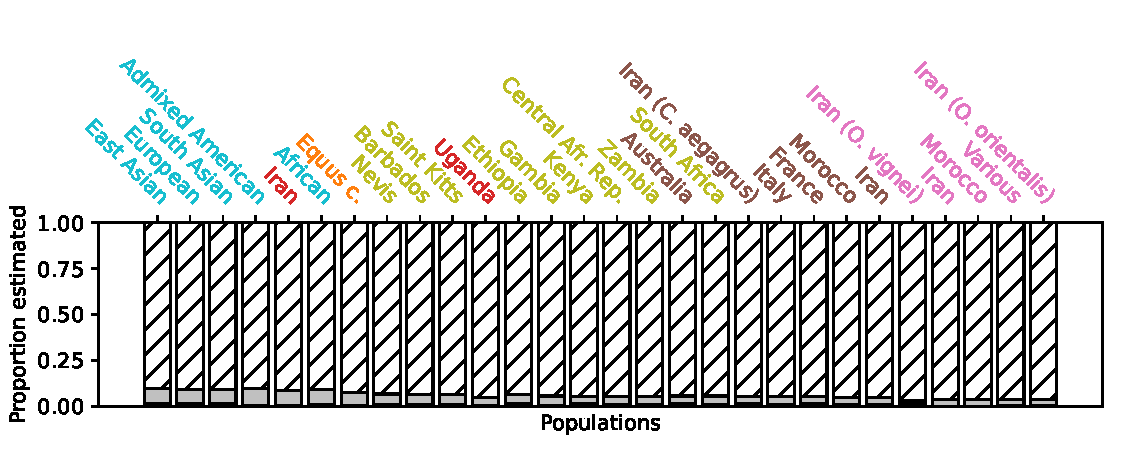
\includegraphics[width=\linewidth, page=1]{artworks/Theta.neg.stacked.pdf}
            \end{minipage}
            \begin{minipage}{0.09\linewidth}
                
\includegraphics[width=\linewidth, page=1]{artworks/legend.polycat}
            \end{minipage}
        \end{minipage}
    \captionof{figure}[Estimation of selection at the population scale for $\SphyDel$ mutations.]{\textbf{Estimation of selection at the population scale for $\bm{\SphyDel}$ mutations.} Each stack bar corresponds to the DFE of new mutations predicted to be $\SphyDel$  by the mutation selection model, in a given population. The dashed area represents the proportion of deleterious mutations ($\SpopDel$), the gray area that of neutral mutations ($\SpopNeu$), and the yellow area that of beneficial mutations ($\SpopBen$).\label{fig:pop-neg}}
    \end{center}


    \begin{center}
        \begin{minipage}{0.75\linewidth}
            \begin{minipage}{0.9\linewidth}
                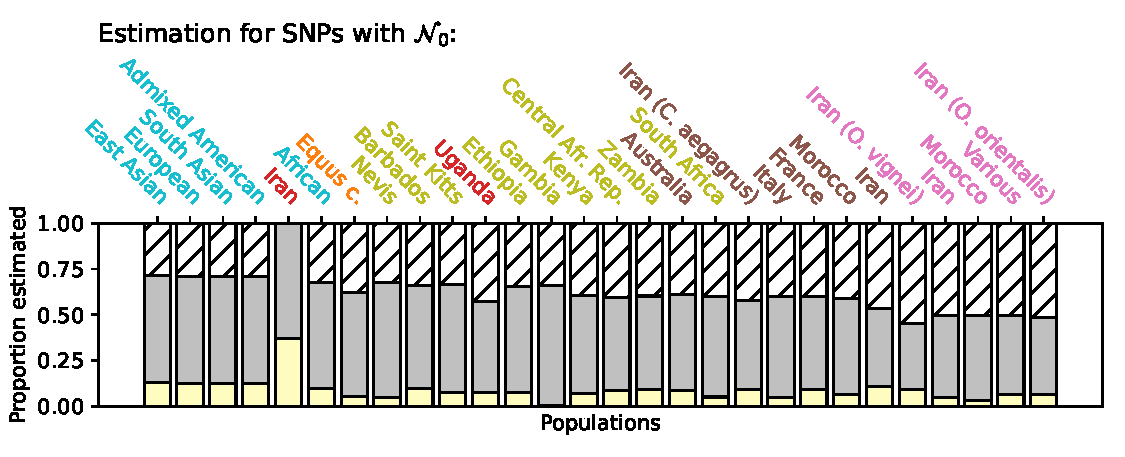
\includegraphics[width=\linewidth, page=1]{artworks/Theta.weak.stacked.pdf}
            \end{minipage}
            \begin{minipage}{0.09\linewidth}
                
\includegraphics[width=\linewidth, page=1]{artworks/legend.polycat}
            \end{minipage}
        \end{minipage}
    \captionof{figure}[Estimation of selection at the population scale for $\SphyNeu$ mutations.]{\textbf{Estimation of selection at the population scale for $\bm{\SphyNeu}$ mutations.} Each stack bar corresponds to the DFE of new mutations predicted to be $\SphyNeu$ by the mutation selection model, in a given population. The dashed area represents the proportion of deleterious mutations ($\SpopDel$), the gray area that of neutral mutations ($\SpopNeu$), and the yellow area that of beneficial mutations ($\SpopBen$).\label{fig:pop-weak}}
    \end{center}


    \begin{center}
        \begin{minipage}{0.75\linewidth}
            \begin{minipage}{0.9\linewidth}
                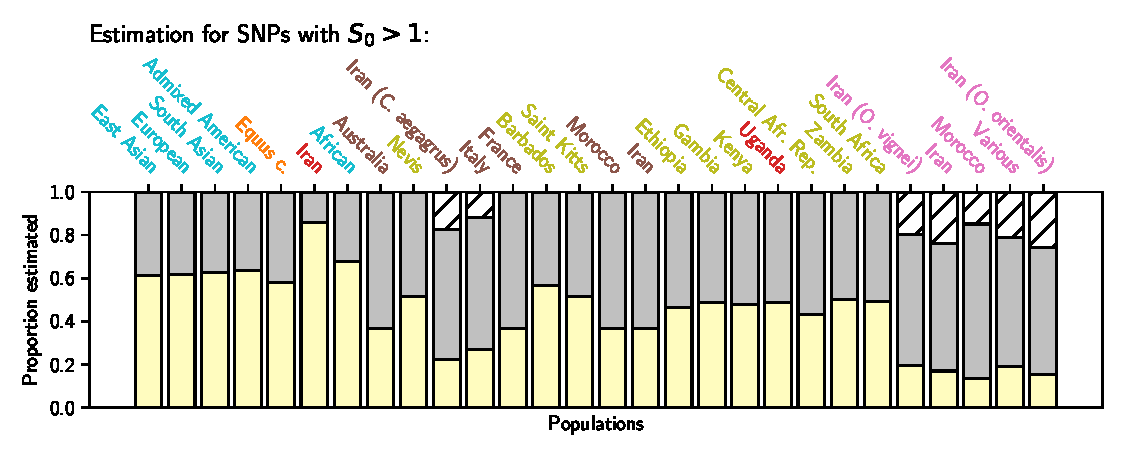
\includegraphics[width=\linewidth, page=1]{artworks/Theta.pos.stacked.pdf}
            \end{minipage}
            \begin{minipage}{0.09\linewidth}
                
\includegraphics[width=\linewidth, page=1]{artworks/legend.polycat}
            \end{minipage}
        \end{minipage}
    \captionof{figure}[Estimation of selection at the population scale for $\SphyBen$ mutations.]{\textbf{Estimation of selection at the population scale for $\bm{\SphyBen}$ mutations.} Each stack bar corresponds to the DFE of new mutations predicted to be $\SphyBen$ by the mutation selection model, in a given population. The dashed area represents the proportion of deleterious mutations ($\SpopDel$), the gray area that of neutral mutations ($\SpopNeu$), and the yellow area that of beneficial mutations ($\SpopBen$).\label{fig:pop-pos}}
    \end{center}

    \newpage
    \subsection{Distribution of scaled selection coefficients (\texorpdfstring{$\Sphy$}{S₀})}\label{subsec:expectedDFE}

    Theoretically, the selection coefficient ($\Sphy$) for any mutation is related to its probability of fixation by the equation $\proba_{\text{fix}} (\Sphy) = \Sphy/(1-\exp(-\Sphy)) $.
    It is thus possible to predict the distribution of $\Sphy$ of substitutions given the distribution of $\Sphy$ for mutations (Figure~\ref{dfe-sfs}A for one population of \textit{Chlorocebus sabaeus}) by weighting the different mutations by their $\proba_{\text{fix}} (\Sphy)$.
    The predicted DFE (distribution of fitness effects) of substitutions (Figure~\ref{dfe-sfs}B) matches the observed DFE of substitutions (Figure~\ref{dfe-sfs}C) in the terminal lineage, meaning that the $\Sphy$ obtained by phylogenetic mutation-selection codon models is a strong predictor of selection effectively exerted on mutations in terminal lineages.
    Equivalent figures to Figure~\ref{dfe-sfs} for each one of the 28 populations are available at Zenodo (\url{https://doi.org/10.5281/zenodo.7878953}) in file \textit{distribution\_S0\_28\_populations.pdf}.\\

    \begin{center}
        \begin{minipage}{0.32\linewidth}
            \flushleft {\tiny A: Expected DFE for mutations}
            \includegraphics[width=\linewidth, page=1]{artworks/DFE.Chlorocebus_sabaeus.Saint_Kitts.MutSel.pdf}
        \end{minipage}
        \begin{minipage}{0.32\linewidth}
            \flushleft {\tiny B: Expected DFE for substitutions}
            \includegraphics[width=\linewidth, page=1]{artworks/DFE.Chlorocebus_sabaeus.Saint_Kitts.MutSel.Flow.pdf}
        \end{minipage}
        \begin{minipage}{0.32\linewidth}
            \flushleft {\tiny C: Observed DFE for substitutions}
            \includegraphics[width=\linewidth, page=1]{artworks/subs.Chlorocebus_sabaeus.Saint_Kitts.bins3Mask0.9.pdf}
        \end{minipage}
        \\
        \begin{minipage}{0.32\linewidth}
            \flushleft {\tiny D: Observed DFE for polymorphisms}
            \includegraphics[width=\linewidth, page=1]{artworks/poly.Chlorocebus_sabaeus.Saint_Kitts.bins3Mask0.9.pdf}
        \end{minipage}
        \begin{minipage}{0.32\linewidth}
            \flushleft {\tiny E: Site frequency spectrum}
            \includegraphics[width=\linewidth, page=1]{artworks/Chlorocebus_sabaeus.Saint_Kitts.MutSel-sfs.normalize.pdf}
        \end{minipage}
        \begin{minipage}{0.32\linewidth}
            \flushleft {\tiny F: $S$ as function of $S_0$ for each class}
            \includegraphics[width=\linewidth, page=1]{artworks/Chlorocebus_sabaeus.Saint_Kitts.MutSel.polyDFE_C.pdf}
        \end{minipage}
        \captionof{figure}[Distribution of scaled selection coefficients ($\Sphy$).]{\textbf{Distribution of scaled selection coefficients ($\bm{\Sphy}$) in the Saint Kitts population of \textit{Chlorocebus sabaeus}.}
        A) Distribution of scaled selection coefficients ($\Sphy$), predicted for all possible non-synonymous DNA mutations away from the ancestral exome.
        Mutations are divided into three classes of selection: deleterious ($\SphyDel$), nearly-neutral ($\SphyNeu$) and beneficial non-adaptive ($\SphyBen$).
        B) Expected distribution of $\Sphy$ for substitutions obtained by transforming the distribution of $\Sphy$ for mutations (panel A) by weighting each mutation by its scaled probability of fixation given by $\proba_{\text{fix}} (\Sphy) = \Sphy/(1-\exp(-\Sphy))$.
        C) Distribution of scaled selection coefficients ($\Sphy$) for all observed substitutions along the terminal branch of the phylogenetic tree.
        D) Distribution of scaled selection coefficients ($\Sphy$) for all observed polymorphisms currently segregating in the population.
        E) The site-frequency spectrum (SFS) in the population for a random sample of 16 alleles (means in solid lines and standard deviations in color shades) for each class of selection and for synonymous mutations, supposedly neutral (black). The SFS represents the proportion of mutations (y-axis) with a given number of derived alleles in the population (x-axis). At high frequencies, deleterious mutations are underrepresented.
        F) Proportion of beneficial $\ProbaPopDel$, nearly-neutral $\ProbaPopNeu$, and deleterious mutations $\ProbaPopBen$  estimated at the population scale for each class of selection at the phylogenetic scale. Proportions depicted here are not weighted by their mutational opportunities.}
        \label{dfe-sfs}
    \end{center}

    \newpage
    \section{Correlation with diversity}

    \subsection{Phylogenetic Generalized Linear Model}

    Because a correlation must account for phylogenetic relationship and non-independence of samples, we fitted a Phylogenetic Generalized Linear Model (PGLM) in R with the package caper~\cite{orme_caper_2013}, with multi-furcation of the different populations inside each species.
    The mammalian tree imported from TimeTree~\cite{kumar_timetree_2017} and pruned to the species used in this study (Figure~\ref{tree}) is shown in newick format:

    \lstinputlisting[breaklines]{artworks/PGLM.tree}

    \begin{center}
        \includegraphics[width=0.65\linewidth, page=1]{artworks/PGLM.pdf}
        \captionof{figure}[Tree used for PGLM (Phylogenetic Generalized Linear Model).]{\textbf{Tree used for PGLM (Phylogenetic Generalized Linear Model).} The mammalian dated tree was obtained from TimeTree~\cite{kumar_timetree_2017} and pruned to include only the species analysed in this study, with multi-furcation of the different populations from each species placed at the same divergence time as the divergence to the sister species.}
        \label{tree}
    \end{center}

    \newpage
    Accounting for phylogenetic relationship and non-independence of samples, through the fit of a Phylogenetic Generalized Linear Model, we can estimate regression coefficient between two variables.
    Thus, for each population, the proportion of deleterious ($\ProbaPopDel$,~\ref{fig:pop-neg-prop}), nearly-neutral ($\ProbaPopNeu$,~\ref{fig:pop-weak-prop}) and beneficial ($\ProbaPopBen$,~\ref{fig:pop-pos-prop}) mutations estimated at the population-genetic scale is shown as function of $\Ne$, and we estimated regression coefficients.


    \subsubsection{Proportion of deleterious mutations (\texorpdfstring{$\SpopDel$}{D})}\label{subsec:proportion-deleterious-mutations}

    Higher effective population size ($\Ne$) is typically accompanied by a higher proportion of effectively deleterious mutations at the population scale ($\proba{[} \SpopDel {]}$), as shown in~\ref{fig:pop-neg-prop} (left panel).
    This trend is also confirmed when we restricted the analysis to class of mutations that are supposedly deleterious at the phylogenetic scale ($\SphyDel$), as shown in~\ref{fig:pop-neg-prop} (right panel).
    This result is qualitatively in accordance with the nearly-neutral theory of evolution which argues that very slightly deleterious mutations are more efficiently purified in large populations.

    \begin{center}
    \begin{minipage}{0.49\linewidth}
        \includegraphics[width=\linewidth, page=1]{artworks/results.pop_size.all_P-Sneg.scatter.pdf}
    \end{minipage}
    \begin{minipage}{0.49\linewidth}
        \includegraphics[width=\linewidth, page=1]{artworks/results.pop_size.neg_P-Sneg.scatter.pdf}
    \end{minipage}
    \captionof{figure}[Relationship between the proportion of deleterious mutations ($\SpopDel$) and effective population size.]{\textbf{Relationship between the proportion of deleterious mutations ($\bm{\SpopDel}$) and effective population size.}
    Left) Proportion of deleterious mutations at the population scale ($\proba{[} \SpopNeu{]}$), shown as a function of estimated effective population size ($\Ne$). Right) Probability for a mutation to be deleterious at the population scale, given it is predicted to be deleterious at the phylogenetic scale, as a function of estimated effective population size ($\Ne$). Populations are represented by circles, and squares are the mean for the species. Correlations account for phylogenetic relationship and non-independence of samples, through the fit of a Phylogenetic Generalized Linear Model (see Materials \& Methods).\label{fig:pop-neg-prop}}
    \end{center}

    \subsubsection{Proportion of nearly-neutral mutations (\texorpdfstring{$\SpopNeu$}{N})}\label{subsec:proportion-nearly-neutral-mutations}
    Higher effective population size ($\Ne$) is typically accompanied by a smaller proportion of neutral mutations at the population scale ($\proba{[} \SpopNeu {]}$ in the range 0.06-0.18), as shown in~\ref{fig:pop-weak-prop} (left panel).
    This result is more pronounced ($\proba{[} \SpopNeu \given \SphyNeu {]}$ in the range 0.36-0.73) when we restricted the analysis to the class of mutations that are supposedly nearly-neutral at the phylogenetic scale ($\SphyNeu$), as shown in~\ref{fig:pop-pos-prop} (right panel).
    This result suggests that in populations with higher diversity (e.g.,~\textit{Bos} or \textit{Ovis}), mutations are more likely to be detected as under selection (positive or negative).
    Alternatively stated, mutations in populations with low diversity (e.g.,~\textit{Homo}) are effectively nearly-neutral and behave as neutral mutations would.
    This result is qualitatively in accordance with the nearly-neutral theory of evolution which argues that mutations are less efficiently selected for in small populations.

    \newpage
    \begin{center}
        \begin{minipage}{0.49\linewidth}
            \includegraphics[width=\linewidth, page=1]{artworks/results.pop_size.all_P-Sweak.scatter.pdf}
        \end{minipage}
        \begin{minipage}{0.49\linewidth}
            \includegraphics[width=\linewidth, page=1]{artworks/results.pop_size.weak_P-Sweak.scatter.pdf}
        \end{minipage}
        \captionof{figure}[Relationship between the proportion of nearly-neutral mutations ($\SpopNeu$) and effective population size.]{\textbf{Relationship between the proportion of nearly-neutral mutations ($\bm{\SpopNeu}$) and effective population size..}
        Left) Proportion of deleterious mutations at the population scale ($\proba{[} \SpopNeu{]}$), shown as a function of estimated effective population size ($\Ne$). Right) Probability for a mutation to be nearly-neutral at the population scale, given it is predicted to be nearly-neutral at the phylogenetic scale, as a function of estimated effective population size ($\Ne$). Populations are represented by circles, and squares are the mean for the species. Correlations account for phylogenetic relationship and non-independence of samples, through the fit of a Phylogenetic Generalized Linear Model (see Materials \& Methods).\label{fig:pop-weak-prop}}
    \end{center}


    \subsubsection{Proportion of beneficial mutations (\texorpdfstring{$\SpopBen$}{B})}\label{subsec:proportion-beneficial-mutations}
    A higher effective population size ($\Ne$) is accompanied by a smaller proportion of beneficial mutations at the population scale ($\proba{[} \SpopBen {]}$), as shown in~\ref{fig:pop-pos-prop} (left panel).
    This trend is also confirmed when we restricted the analysis to the class of mutations that are supposedly non-adaptive beneficial at the phylogenetic scale ($\SphyBen$), as shown in~\ref{fig:pop-pos-prop} (right panel).


    \begin{center}
        \begin{minipage}{0.49\linewidth}
            \includegraphics[width=\linewidth, page=1]{artworks/results.pop_size.all_P-Spos.scatter.pdf}
        \end{minipage}
        \begin{minipage}{0.49\linewidth}
            \includegraphics[width=\linewidth, page=1]{artworks/results.pop_size.pos_P-Spos.scatter.pdf}
        \end{minipage}
        \captionof{figure}[Relationship between the proportion of beneficial mutations ($\SpopBen$) and effective population size.]{\textbf{Relationship between the proportion of beneficial mutations ($\bm{\SpopBen}$) and effective population size.}
        Left) Proportion of beneficial mutations at the population scale ($\proba{[} \SpopNeu{]}$), shown as a function of estimated effective population size ($\Ne$). Right) Probability for a mutation to be beneficial at the population scale, given it is predicted to be beneficial at the phylogenetic scale, as a function of estimated effective population size ($\Ne$). Populations are represented by circles, and squares are the mean for the species. Correlations account for phylogenetic relationship and non-independence of samples, through the fit of a Phylogenetic Generalized Linear Model (see Materials \& Methods).\label{fig:pop-pos-prop}}
    \end{center}


    \newpage

    \section{Probability for beneficial mutations to be non-adaptive (\texorpdfstring{$\proba{[}\SphyBen\given \SpopBen {]}$}{P[B₀|B]})}

    \subsection{Across different populations}
    Probability for beneficial mutations to be non-adaptive, namely $\proba{[}\SphyBen\given \SpopBen {]}$, is obtained from Bayes' formula (eq.~14) merging three terms: the probability for a new mutation to be a non-adaptive beneficial mutation ($\proba{[} \SphyBen {]}$, eq.~5), the probability for a mutation to be beneficial ($\proba{[} \SpopBen {]}$, eq.~15) and the probability for a mutation to be beneficial at the population scale given that it is predicted to be a non-adaptive beneficial mutation at the phylogenetic scale ($\proba{[} \SpopBen \given \SphyBen{]}$, eq.~12).
    These four estimates across populations are shown in Table~\ref{table:proba}.

    \begin{center}
        \scriptsize
        \begin{longtable*}{|l|l|r|r|r|r|r|r|}
            \toprule
            Population & Species & $N_e$ & $\proba{[}\SphyBen{]}$ & $\proba{[} \SpopBen {]}$ & $\frac{\proba{[}\SphyBen]}{\proba{[} \SpopBen ]}$ & $\proba{[} \SpopBen \given \SphyBen{]}$ & $\proba{[}\SphyBen\given \SpopBen {]}$ \\
            \midrule
            \endhead
            \midrule
            \multicolumn{8}{r}{{Continued on next page}} \\
            \midrule
            \endfoot
            \bottomrule
            \endlastfoot
            \rowcolor{LIGHTGREY} Equus c. & Equus caballus & $7.5\times 10^{4}$ & $ 0.012$ & $ 0.015$ & $ 0.827$ & $ 0.648$ & $ 0.536$ \\
            Iran & Bos taurus & $5.6\times 10^{4}$ & $ 0.011$ & $ 0.039$ & $ 0.279$ & $ 0.873$ & $ 0.243$ \\
            Uganda & Bos taurus & $1.3\times 10^{5}$ & $ 0.011$ & $ 0.015$ & $ 0.720$ & $ 0.576$ & $ 0.415$ \\
            \rowcolor{LIGHTGREY} Australia & Capra hircus & $1.7\times 10^{5}$ & $ 0.011$ & $ 0.023$ & $ 0.480$ & $ 0.368$ & $ 0.177$ \\
            \rowcolor{LIGHTGREY} France & Capra hircus & $1.9\times 10^{5}$ & $ 0.011$ & $ 0.022$ & $ 0.515$ & $ 0.368$ & $ 0.190$ \\
            \rowcolor{LIGHTGREY} Iran (C. aegagrus) & Capra hircus & $1.9\times 10^{5}$ & $ 0.011$ & $ 0.025$ & $ 0.448$ & $ 0.368$ & $ 0.165$ \\
            \rowcolor{LIGHTGREY} Iran & Capra hircus & $2.3\times 10^{5}$ & $ 0.011$ & $ 0.021$ & $ 0.525$ & $ 0.368$ & $ 0.193$ \\
            \rowcolor{LIGHTGREY} Italy & Capra hircus & $1.9\times 10^{5}$ & $ 0.011$ & $ 0.017$ & $ 0.660$ & $ 0.368$ & $ 0.243$ \\
            \rowcolor{LIGHTGREY} Morocco & Capra hircus & $2.2\times 10^{5}$ & $ 0.011$ & $ 0.017$ & $ 0.667$ & $ 0.368$ & $ 0.245$ \\
            Iran & Ovis aries & $3.8\times 10^{5}$ & $ 0.012$ & $ 0.006$ & $ 1.984$ & $ 0.205$ & $ 0.407$ \\
            Iran (O. orientalis) & Ovis aries & $4.5\times 10^{5}$ & $ 0.011$ & $ 0.012$ & $ 0.983$ & $ 0.193$ & $ 0.190$ \\
            Iran (O. vignei) & Ovis aries & $3.7\times 10^{5}$ & $ 0.012$ & $ 0.020$ & $ 0.579$ & $ 0.190$ & $ 0.110$ \\
            Various & Ovis aries & $4.1\times 10^{5}$ & $ 0.011$ & $ 0.012$ & $ 0.967$ & $ 0.229$ & $ 0.222$ \\
            Morocco & Ovis aries & $ 4\times 10^{5}$ & $ 0.012$ & $ 0.005$ & $ 2.435$ & $ 0.211$ & $ 0.514$ \\
            \rowcolor{LIGHTGREY} Barbados & Chlorocebus sabaeus & $1.1\times 10^{5}$ & $ 0.009$ & $ 0.021$ & $ 0.452$ & $ 0.648$ & $ 0.293$ \\
            \rowcolor{LIGHTGREY} Central Afr. Rep. & Chlorocebus sabaeus & $1.7\times 10^{5}$ & $ 0.009$ & $ 0.018$ & $ 0.515$ & $ 0.535$ & $ 0.275$ \\
            \rowcolor{LIGHTGREY} Ethiopia & Chlorocebus sabaeus & $1.4\times 10^{5}$ & $ 0.009$ & $ 0.021$ & $ 0.444$ & $ 0.552$ & $ 0.245$ \\
            \rowcolor{LIGHTGREY} Gambia & Chlorocebus sabaeus & $1.4\times 10^{5}$ & $ 0.009$ & $ 0.007$ & $ 1.423$ & $ 0.577$ & $ 0.821$ \\
            \rowcolor{LIGHTGREY} Kenya & Chlorocebus sabaeus & $1.5\times 10^{5}$ & $ 0.009$ & $ 0.022$ & $ 0.437$ & $ 0.588$ & $ 0.257$ \\
            \rowcolor{LIGHTGREY} Nevis & Chlorocebus sabaeus & $ 1\times 10^{5}$ & $ 0.009$ & $ 0.016$ & $ 0.597$ & $ 0.599$ & $ 0.358$ \\
            \rowcolor{LIGHTGREY} South Africa & Chlorocebus sabaeus & $1.8\times 10^{5}$ & $ 0.009$ & $ 0.016$ & $ 0.594$ & $ 0.574$ & $ 0.341$ \\
            \rowcolor{LIGHTGREY} Saint Kitts & Chlorocebus sabaeus & $1.2\times 10^{5}$ & $ 0.009$ & $ 0.017$ & $ 0.563$ & $ 0.598$ & $ 0.336$ \\
            \rowcolor{LIGHTGREY} Zambia & Chlorocebus sabaeus & $1.7\times 10^{5}$ & $ 0.009$ & $ 0.022$ & $ 0.427$ & $ 0.585$ & $ 0.250$ \\
            African & Homo sapiens & $5.6\times 10^{4}$ & $ 0.010$ & $ 0.020$ & $ 0.484$ & $ 0.721$ & $ 0.349$ \\
            Admixed American & Homo sapiens & $4.5\times 10^{4}$ & $ 0.010$ & $ 0.019$ & $ 0.500$ & $ 0.690$ & $ 0.345$ \\
            East Asian & Homo sapiens & $ 4\times 10^{4}$ & $ 0.010$ & $ 0.027$ & $ 0.362$ & $ 0.688$ & $ 0.249$ \\
            European & Homo sapiens & $4.2\times 10^{4}$ & $ 0.010$ & $ 0.027$ & $ 0.361$ & $ 0.688$ & $ 0.248$ \\
            South Asian & Homo sapiens & $4.4\times 10^{4}$ & $ 0.010$ & $ 0.030$ & $ 0.324$ & $ 0.691$ & $ 0.224$ \\
        \end{longtable*}
        \captionof{table}[Probability for beneficial mutations to be non-adaptive ($\proba{[}\SphyBen\given \SpopBen {]}$)]{
        \textbf{Probability for beneficial mutations to be non-adaptive ($\bm{\proba{[}\SphyBen\given \SpopBen {]}}$).}
        $\Ne$ is the estimated effective population size.
        $\proba{[} \SphyBen {]}$ (eq.~5) is the probability for a new mutation to be a non-adaptive beneficial mutation.
        These mutations have a selection coefficient predicted at the phylogenetic-scale larger than 1, thus toward a more fit amino-acid.
        $\proba{[} \SpopBen {]}$ (eq.~15) is the probability for a mutation to be beneficial.
        These mutations have a selection coefficient at the population-scale larger than 1.
        $\proba{[} \SpopBen \given \SphyBen{]}$ (eq.~12) is the probability for a mutation to be beneficial at the population scale, given that it is predicted to be a non-adaptive beneficial mutation at the phylogenetic scale (the \textit{precision}).
        $\proba{[} \SphyBen \given \SpopBen{]}$ (eq.~14) is the probability for a mutation to be non-adaptive given that it is beneficial at the population scale (the \textit{recall}).
        This probability is obtained using Bayes' formula.
        \label{table:proba}
        }
    \end{center}

    \newpage
    \subsection{Misannotations of ancestral alleles}

    A potential caveat of our method is that if a deleterious derived allele segregates at low frequency but is wrongly annotated as ancestral, it will result in a SNP that will be both predicted as advantageous and segregating at high frequency, wrongly suggesting that this variant is correctly inferred as beneficial.
    In this context, misannotations of ancestral alleles could inflate our estimation of the proportion of beneficial non-adaptive mutations.
    However, we show that this problem impacts our estimation in two ways, albeit, only slightly. \\

    First, if misannotation is influencing the recall for $\SphyBen$ ($\proba{[}\SphyBen\given \SpopBen {]}$), then the recall should increase as a function of  divergence to the sister species ($\ds$: number of synonymous substitutions per site) since divergence would increase the rate of misannotations.
    Shown in Figure~\ref{fig:distance-sister} is recall $\proba{[}\SphyBen\given \SpopBen {]}$ as a function of divergence ($\ds$) in which the latter is not an explanatory variable.

    \begin{center}
        \includegraphics[width=0.75\linewidth, page=1]{artworks/results.distance.recall_pos.scatter.pdf}
        \captionof{figure}[$\proba{[}\SphyBen\given \SpopBen {]}$ as a function of distance to the sister species.]{\textbf{Proportion of non-adaptive mutations among beneficial ones ($\bm{\proba{[}\SphyBen\given \SpopBen {]}}$) as a function of distance to the sister species.}
        $\proba{[} \SphyBen \given \SpopBen{]}$ (eq.~14) is the probability for a beneficial mutation to be non-adaptive.
        $\ds$ is number of synonymous substitutions per site that occurred since divergence with the sister species (closest species in the mammalian tree).
        Populations are represented by circles, and squares are the mean for the species.
        Correlations account for phylogenetic relationship and non-independence of samples, through the fit of a Phylogenetic Generalized Linear Model (see Materials \& Methods).\label{fig:distance-sister}}
    \end{center}

    \newpage

    Second, the distribution of selection coefficients ($\Sphy$) that we observed for segregating mutations and for divergence also suggests that we effectively controlled for misannotations.
    Under a scenario where beneficial non-adaptive mutations would only be the result of misannotations, one would expect that the positive part of the fitness effects ($\proba{[}\Sphy{]}$) of observed polymorphisms currently segregating in the population should reflect the negative one ($\proba{[}-\Sphy{]}$).
    Indeed, the number of misannotated beneficial mutations should be proportional to the number of deleterious mutations with the same selection coefficient.
    The ratio between advantageous and deleterious polymorphisms of the same selection coefficient should therefore be a constant that represents the rate of misannotation (typically influenced by the distance to the sister species).
    However, this is not what we observe in the DFE of polymorphisms (shown in Figure~\ref{mispol-expectation} for the African population of \textit{Homo sapiens}) thus giving us the confidence that misannotations are not common.
    Overall, the observed DFE of substitutions is much better explained by the expected DFE of new mutations (section S\ref{subsec:expectedDFE} than by misannotations).


    \begin{center}
        \includegraphics[width=0.75\linewidth, page=1]{artworks/poly.Homo_sapiens.AFR.folded_ratio.pdf}
        \captionof{figure}[Ratio of $\proba{[}\Sphy{]}$ over $\proba{[}-\Sphy{]}$ for polymorphisms of the African population of \textit{Homo sapiens}.]{\textbf{Ratio of $\bm{\proba{[}\Sphy{]}}$ over $\bm{\proba{[}-\Sphy{]}}$ for polymorphisms of the African population of \textit{Homo sapiens}.}
        From the histogram of distribution of scaled selection coefficients ($\Sphy$) for all observed polymorphism, we obtain 30 bins for positive selection coefficient ($\Sphy$) and 30 bins for negative selection coefficient ($\Sphy$). For a given bin of $\Sphy$, $\proba{[}\Sphy{]}$ the number of observed polymorphisms in the positive part, while $\proba{[}-\Sphy{]}$ the number of observed polymorphisms in the negative part. $\bm{\proba{[}\Sphy{]} / \proba{[}-\Sphy{]}}$ is the ratio of the positive part over the negative part. Alternatively stated, it is folding Figure~\ref{dfe-sfs}D around 0, by taking the right part (positive $\Sphy$) of the histogram over the left part (negative $\Sphy$).
        }
        \label{mispol-expectation}
    \end{center}

    \newpage
    \subsection{Simulations of site-frequency spectra}

    We performed population-genetic simulations to test whether our approach is able to recover the proportion of beneficial mutations that are non-adaptive in synthetic polymorphism datasets.
    More specifically, we performed simulations of site-frequency spectra, thus at the population-genetic scale, by using a mixture of the DFEs that is predicted from the phylogenetic mutation-selection model, and adding adaptive mutations to this DFE.
    In practice, simulations are performed under the Poisson Random Field (PRF) framework of population genetics\cite{sawyer_population_1992}.
    Each simulation generates a synthetic synonymous SFS, and a synthetic non-synonymous SFS for the mutations in the category $x \in \{ \SphyDel, \SphyNeu, \SphyBen \}$.

    Technically, for non-synonymous mutations, we first draw a random sample of the selection coefficients from the mixture of DFEs using $\proba{[}y \given x{]}$ for $y \in \{ \SpopDel, \SpopNeu, \SpopBen \}$ as parameters.
    Importantly, $\proba{[}\SpopBen \given \SphyDel{]}$ and $\proba{[}\SpopBen \given \SphyNeu{]}$ are considered adaptive mutations, and thus their selection coefficients have a selection coefficient of $S_{\text{adaptive}}=10$.
    All the others are drawn for the DFEs that are predicted from the phylogenetic mutation-selection model.
    Synonymous mutations are considered neutral and have $S=0$.

    Given these selection coefficients, to obtain the expected SFS we integrate over the limiting density of frequency that mutations are segregating in the population, as described from eqs. 1--2 in \textcite{tataru_inference_2017}.
    And finally, given this expected SFS, we perform a Poisson random sampling to obtain a sampled SFS of size n matching the total number of polymorphism to simulate.

    In summary, the simulations generates a synonymous SFS, and a non-synonymous SFS for the mutations in the category $x \in \{ \SphyDel, \SphyNeu, \SphyBen \}$, and require as input the following:
    \begin{itemize}
        \item Total number of polymorphisms to simulate (synonymous and non-synonymous).
        \item The DFE of $\Sphy$ predicted from the phylogenetic mutation-selection.
        \item Estimates of $\proba{[}y \given x{]}$ for $y \in \{ \SpopDel, \SpopNeu, \SpopBen \}$.
        \item Selection coefficient for adaptive mutations, here $S_{\text{adaptive}}=20$.
        \item The sampled SFS size $n$, here $n=16$ (i.e.\ twice the number of sampled individuals).
    \end{itemize}

    From these two SFS (synonymous and non-synonymous), we run polyDFE to obtain $\proba{[}\SpopDel \given x{]}$, $\proba{[}\SpopNeu \given x{]}$ and $\proba{[}\SpopBen \given x{]}$ (eqs.\ 9--11).
    By doing so for the 3 categories $x \in \{ \SphyDel, \SphyNeu, \SphyBen \}$, we can ultimately compute $\proba{[}\SphyBen \given \SpopBen{]}$ (eqs.\ 14--15), which can be then be compared to the ground truth.

    We used 8 different sets of parameters ($\proba{[}y \given x{]}$ and number of polymorphisms) and simulated 10 replicates for each set of parameters, shown in Figure~\ref{fig:simulations}.
    These set of input parameters are provided to match $\proba{[}\SphyBen \given \SpopBen{]}$ of the following populations: Set 1 for Admixed American (\textit{Homo sapiens}), Set 2 for African (\textit{Homo sapiens}), Set 3 for Nevis (\textit{Chlorocebus sabaeus}), Set 4 for Iran (\textit{Ovis orientalis}), Set 5 for Uganda (\textit{Bos taurus}), Set 6 for Morocco (\textit{Ovis aries}), Set 7 for \textit{Equus caballus}, Set 8 for Gambia (\textit{Chlorocebus sabaeus}).
    For each synthetic data we ran polyDFE and derived $\proba{[}\SphyBen \given \SpopBen{]}$ which was then compared to the ground truth (calculated analytically from the set parameters $\proba{[}y \given x], x \in \{ \SphyDel, \SphyNeu, \SphyBen \}, y \in \{ \SpopDel, \SpopNeu, \SpopBen \}$).
    These simulations show that we are able to accurately retrieve the proportion of non-adaptive mutations in those synthetic datasets.


    \begin{center}
        \includegraphics[width=\linewidth, page=1]{artworks/simulations.pos.pdf}
        \captionof{figure}[Proportion of non-adaptive mutations among beneficial ones ($\proba{[}\SphyBen\given \SpopBen {]}$) estimated on synthetic site-frequency spectra.]{\textbf{Proportion of non-adaptive mutations among beneficial ones ($\bm{\proba{[}\SphyBen\given \SpopBen {]}}$) estimated on synthetic site-frequency spectra.} Each set has ben simulated using a different value for $\proba{[}\SphyBen\given \SpopBen {]}$. Bars correspond to the $\proba{[}\SphyBen\given \SpopBen {]}$ used to simulate the site-frequency spectra, each blue circle corresponds to $\proba{[}\SphyBen\given \SpopBen {]}$ estimated by one polyDFE simulation, and red crosses correspond to the mean of estimations across 10 replicates.\label{fig:simulations}}
    \end{center}


    \section{Filtering of variable sites}

    \subsection{Masking CpG transitions}
    We also tested our prediction when masking CpG transitions since the mutation rate of CpG dinucleotides is higher than the mutation rate of other dinucleotides, which can affect the estimation of the DFE.
    Any nucleotide transition including a CpG dinucleotide either in the ancestral or derived state is considered as a CpG transition.
    We masked all CpG transitions in the mutational opportunities, the substitutions in the terminal branches, and the polymorphisms segregating in the population. We then re-estimated the DFE and the proportion of non-adaptive beneficial mutations.

    \newpage
    \subsection{Probability for beneficial mutations to be non-adaptive}
    When filtering out CpG sites, the estimation of $\proba{[} \SpopBen {]}$ and $\proba{[}\SphyBen\given \SpopBen {]}$ across populations is shown in Table~\ref{table:no-CpG-bayes}.
    Comparing these results with Table~\ref{table:proba}, we acknowledge that the exact proportion of non-adaptive among beneficial mutations is dependent on the whether we masked CpG sites.
    However, we can still see that non-adaptive beneficial mutations are positively selected compared to neutral and deleterious ones, and this result is not dependent on whether we masked CpG sites or not.

    \begin{center}
        \scriptsize
        \begin{longtable*}{|l|l|r|r|r|r|r|r|}
            \toprule
            Population & Species & $\Ne$ & $\proba{[}\SphyBen{]}$ & $\proba{[} \SpopBen {]}$ & $\frac{\proba{[}\SphyBen]}{\proba{[} \SpopBen ]}$ & $\proba{[} \SpopBen \given \SphyBen{]}$ & $\proba{[}\SphyBen\given \SpopBen {]}$ \\
            \midrule
            \endhead
            \midrule
            \multicolumn{8}{r}{{Continued on next page}} \\
            \midrule
            \endfoot

            \bottomrule
            \endlastfoot
            \rowcolor{LIGHTGREY} Equus c. & Equus caballus & $7.5\times 10^{4}$ & $ 0.012$ & $ 0.028$ & $ 0.421$ & $ 0.543$ & $ 0.229$ \\
            Iran & Bos taurus & $5.6\times 10^{4}$ & $ 0.011$ & $ 0.038$ & $ 0.283$ & $ 0.797$ & $ 0.226$ \\
            Uganda & Bos taurus & $1.3\times 10^{5}$ & $ 0.011$ & $ 0.022$ & $ 0.479$ & $ 0.406$ & $ 0.195$ \\
            \rowcolor{LIGHTGREY} Australia & Capra hircus & $1.7\times 10^{5}$ & $ 0.011$ & $ 0.024$ & $ 0.454$ & $ 0.158$ & $ 0.072$ \\
            \rowcolor{LIGHTGREY} France & Capra hircus & $1.9\times 10^{5}$ & $ 0.011$ & $ 0.034$ & $ 0.320$ & $ 0.258$ & $ 0.082$ \\
            \rowcolor{LIGHTGREY} Iran (C. aegagrus) & Capra hircus & $1.9\times 10^{5}$ & $ 0.011$ & $ 0.032$ & $ 0.341$ & $ 0.268$ & $ 0.091$ \\
            \rowcolor{LIGHTGREY} Iran & Capra hircus & $2.3\times 10^{5}$ & $ 0.011$ & $ 0.026$ & $ 0.417$ & $ 0.294$ & $ 0.123$ \\
            \rowcolor{LIGHTGREY} Italy & Capra hircus & $1.9\times 10^{5}$ & $ 0.011$ & $ 0.023$ & $ 0.472$ & $ 0.100$ & $ 0.047$ \\
            \rowcolor{LIGHTGREY} Morocco & Capra hircus & $2.2\times 10^{5}$ & $ 0.011$ & $ 0.018$ & $ 0.593$ & $ 0.141$ & $ 0.083$ \\
            Iran & Ovis aries & $3.8\times 10^{5}$ & $ 0.011$ & $ 0.012$ & $ 0.981$ & $ 0.243$ & $ 0.239$ \\
            Iran (O. orientalis) & Ovis aries & $4.5\times 10^{5}$ & $ 0.011$ & $ 0.019$ & $ 0.603$ & $ 0.155$ & $ 0.093$ \\
            Iran (O. vignei) & Ovis aries & $3.7\times 10^{5}$ & $ 0.011$ & $ 0.025$ & $ 0.445$ & $ 0.252$ & $ 0.112$ \\
            Various & Ovis aries & $4.1\times 10^{5}$ & $ 0.011$ & $ 0.016$ & $ 0.704$ & $ 0.198$ & $ 0.139$ \\
            Morocco & Ovis aries & $ 4\times 10^{5}$ & $ 0.011$ & $ 0.008$ & $ 1.389$ & $ 0.165$ & $ 0.229$ \\
            \rowcolor{LIGHTGREY} Barbados & Chlorocebus sabaeus & $1.1\times 10^{5}$ & $ 0.009$ & $ 0.013$ & $ 0.752$ & $ 0.231$ & $ 0.174$ \\
            \rowcolor{LIGHTGREY} Central Afr. Rep. & Chlorocebus sabaeus & $1.7\times 10^{5}$ & $ 0.009$ & $ 0.018$ & $ 0.519$ & $ 0.209$ & $ 0.108$ \\
            \rowcolor{LIGHTGREY} Ethiopia & Chlorocebus sabaeus & $1.4\times 10^{5}$ & $ 0.009$ & $ 0.025$ & $ 0.385$ & $ 0.241$ & $ 0.093$ \\
            \rowcolor{LIGHTGREY} Gambia & Chlorocebus sabaeus & $1.4\times 10^{5}$ & $ 0.009$ & $ 0.007$ & $ 1.346$ & $ 0.204$ & $ 0.275$ \\
            \rowcolor{LIGHTGREY} Kenya & Chlorocebus sabaeus & $1.5\times 10^{5}$ & $ 0.009$ & $ 0.021$ & $ 0.443$ & $ 0.239$ & $ 0.106$ \\
            \rowcolor{LIGHTGREY} Nevis & Chlorocebus sabaeus & $ 1\times 10^{5}$ & $ 0.009$ & $ 0.014$ & $ 0.690$ & $ 0.146$ & $ 0.101$ \\
            \rowcolor{LIGHTGREY} South Africa & Chlorocebus sabaeus & $1.8\times 10^{5}$ & $ 0.009$ & $ 0.019$ & $ 0.498$ & $ 0.272$ & $ 0.135$ \\
            \rowcolor{LIGHTGREY} Saint Kitts & Chlorocebus sabaeus & $1.2\times 10^{5}$ & $ 0.009$ & $ 0.017$ & $ 0.567$ & $ 0.217$ & $ 0.123$ \\
            \rowcolor{LIGHTGREY} Zambia & Chlorocebus sabaeus & $1.7\times 10^{5}$ & $ 0.009$ & $ 0.024$ & $ 0.388$ & $ 0.308$ & $ 0.119$ \\
            African & Homo sapiens & $5.6\times 10^{4}$ & $ 0.010$ & $ 0.026$ & $ 0.367$ & $ 0.411$ & $ 0.151$ \\
            Admixed American & Homo sapiens & $4.5\times 10^{4}$ & $ 0.010$ & $ 0.017$ & $ 0.551$ & $ 0.374$ & $ 0.206$ \\
            East Asian & Homo sapiens & $ 4\times 10^{4}$ & $ 0.010$ & $ 0.029$ & $ 0.332$ & $ 0.370$ & $ 0.123$ \\
            European & Homo sapiens & $4.2\times 10^{4}$ & $ 0.010$ & $ 0.031$ & $ 0.304$ & $ 0.371$ & $ 0.113$ \\
            South Asian & Homo sapiens & $4.4\times 10^{4}$ & $ 0.010$ & $ 0.032$ & $ 0.302$ & $ 0.369$ & $ 0.111$ \\
        \end{longtable*}
        \captionof{table}[$\proba{[}\SphyBen\given \SpopBen {]}$ when masking CpG transitions.]{\textbf{$\bm{\proba{[}\SphyBen\given \SpopBen {]}}$ when masking CpG transitions.}
        $\Ne$ is the estimated effective population size.
        $\proba{[} \SphyBen {]}$ (eq.~5) is the probability for a new mutation to be a non-adaptive beneficial mutation.
        These mutations have a selection coefficient predicted at the phylogenetic-scale larger than 1, thus toward a more fit amino-acid.
        $\proba{[} \SpopBen {]}$ (eq.~15) is the probability for a mutation to be beneficial.
        These mutations have a selection coefficient at the population-scale larger than 1.
        $\proba{[} \SpopBen \given \SphyBen{]}$ (eq.~12) is the probability for a mutation to be beneficial at the population scale, given it is predicted to be a non-adaptive beneficial mutation at the phylogenetic scale (the \textit{precision}).
        $\proba{[} \SphyBen \given \SpopBen{]}$ (eq.~14) is the probability for a mutation to be non-adaptive given it is beneficial at the population scale (the \textit{recall}).
        This probability is obtained using Bayes' formula.\label{table:no-CpG-bayes}}
    \end{center}

    \newpage

    \subsection{Precision and recall}
    The estimation of precision and recall across populations while filtering out CpG sites for the estimation of $\Spop$ is shown in Table~\ref{table:no-CpG}.
    Comparing these results with tables 1, we acknowledge that the exact quantification of \textit{precision} and \textit{recall} is dependent on the whether we masked CpG sites.
    However, we can still see that non-adaptive beneficial mutations are positively selected compared to neutral and deleterious ones, and this result is not dependent on whether we masked CpG sites or not.
    \begin{center}
        \begin{adjustbox}{width=\textwidth}
            \begin{tabular}{||l|l|r||r|r||r|r||r|r||}
                \toprule
                \multicolumn{3}{||c||}{} &
                \multicolumn{2}{c||}{\shortstack{\textbf{Deleterious mutations} \\ $\bm{\SpopDel \coloneqq \Spop<-1}$ \\ $\bm{\SphyDel \coloneqq \Sphy<-1}$}} &
                \multicolumn{2}{c||}{\shortstack{\textbf{Nearly-neutral mutations} \\ $\bm{\SpopNeu \coloneqq -1<\Spop<1}$ \\ $\bm{\SphyNeu \coloneqq -1<\Sphy<1}$}} &
                \multicolumn{2}{c||}{\shortstack{\textbf{Beneficial mutations} \\ $\bm{\SpopBen \coloneqq \Spop>1}$ \\ $\bm{\SphyBen \coloneqq \Sphy>1}$}}
                \\ \hline
                \textbf{Population} &
                \textbf{Species} &
                $\bm{\Ne}$ &
                \makecell{\textbf{Precision} \\ $\bm{\proba{[}\SpopDel \given \SphyDel]}$} &
                \makecell{\textbf{Recall} \\ $\bm{\proba{[}\SphyDel \given \SpopDel]}$}           &
                \makecell{\textbf{Precision}      \\ $\bm{\proba{[}\SpopNeu \given \SphyNeu]}$}                                    &
                \makecell{\textbf{Recall}          \\ $\bm{\proba{[}\SphyNeu \given \SpopNeu]}$}                                  &
                \makecell{\textbf{Precision}          \\ $\bm{\proba{[}\SpopBen \given \SphyBen]}$}          &
                \makecell{\textbf{Recall}        \\ $\bm{\proba{[}\SphyBen \given \SpopBen]}$}
                \\   \midrule
                \rowcolor{LIGHTGREY} Equus c. & Equus caballus & $7.5\times 10^{4}$ & $ 0.887$ & $ 0.984$ & $ 0.740$ & $ 0.356$ & $ 0.543$ & $ 0.229$ \\
                Iran & Bos taurus & $5.6\times 10^{4}$ & $ 0.888$ & $ 1.000$ & $ 0.632$ & $ 0.302$ & $ 0.797$ & $ 0.226$ \\
                Uganda & Bos taurus & $1.3\times 10^{5}$ & $ 0.929$ & $ 0.973$ & $ 0.501$ & $ 0.349$ & $ 0.406$ & $ 0.195$ \\
                \rowcolor{LIGHTGREY} Australia & Capra hircus & $1.7\times 10^{5}$ & $ 0.926$ & $ 0.972$ & $ 0.609$ & $ 0.421$ & $ 0.158$ & $ 0.072$ \\
                \rowcolor{LIGHTGREY} France & Capra hircus & $1.9\times 10^{5}$ & $ 0.927$ & $ 0.959$ & $ 0.354$ & $ 0.321$ & $ 0.258$ & $ 0.082$ \\
                \rowcolor{LIGHTGREY} Iran (C. aegagrus) & Capra hircus & $1.9\times 10^{5}$ & $ 0.931$ & $ 0.967$ & $ 0.502$ & $ 0.423$ & $ 0.268$ & $ 0.091$ \\
                \rowcolor{LIGHTGREY} Iran & Capra hircus & $2.3\times 10^{5}$ & $ 0.937$ & $ 0.966$ & $ 0.529$ & $ 0.451$ & $ 0.294$ & $ 0.123$ \\
                \rowcolor{LIGHTGREY} Italy & Capra hircus & $1.9\times 10^{5}$ & $ 0.927$ & $ 0.970$ & $ 0.550$ & $ 0.390$ & $ 0.100$ & $ 0.047$ \\
                \rowcolor{LIGHTGREY} Morocco & Capra hircus & $2.2\times 10^{5}$ & $ 0.933$ & $ 0.965$ & $ 0.534$ & $ 0.401$ & $ 0.141$ & $ 0.083$ \\
                Iran & Ovis aries & $3.8\times 10^{5}$ & $ 0.947$ & $ 0.957$ & $ 0.446$ & $ 0.393$ & $ 0.243$ & $ 0.239$ \\
                Iran (O. orientalis) & Ovis aries & $4.5\times 10^{5}$ & $ 0.951$ & $ 0.961$ & $ 0.396$ & $ 0.386$ & $ 0.155$ & $ 0.093$ \\
                Iran (O. vignei) & Ovis aries & $3.7\times 10^{5}$ & $ 0.954$ & $ 0.960$ & $ 0.379$ & $ 0.432$ & $ 0.252$ & $ 0.112$ \\
                Various & Ovis aries & $4.1\times 10^{5}$ & $ 0.949$ & $ 0.956$ & $ 0.434$ & $ 0.418$ & $ 0.198$ & $ 0.139$ \\
                Morocco & Ovis aries & $ 4\times 10^{5}$ & $ 0.946$ & $ 0.959$ & $ 0.453$ & $ 0.374$ & $ 0.165$ & $ 0.229$ \\
                \rowcolor{LIGHTGREY} Barbados & Chlorocebus sabaeus & $1.1\times 10^{5}$ & $ 0.916$ & $ 0.971$ & $ 0.523$ & $ 0.306$ & $ 0.231$ & $ 0.174$ \\
                \rowcolor{LIGHTGREY} Central Afr. Rep. & Chlorocebus sabaeus & $1.7\times 10^{5}$ & $ 0.933$ & $ 0.969$ & $ 0.486$ & $ 0.353$ & $ 0.209$ & $ 0.108$ \\
                \rowcolor{LIGHTGREY} Ethiopia & Chlorocebus sabaeus & $1.4\times 10^{5}$ & $ 0.918$ & $ 0.973$ & $ 0.533$ & $ 0.348$ & $ 0.241$ & $ 0.093$ \\
                \rowcolor{LIGHTGREY} Gambia & Chlorocebus sabaeus & $1.4\times 10^{5}$ & $ 0.925$ & $ 0.971$ & $ 0.572$ & $ 0.343$ & $ 0.204$ & $ 0.275$ \\
                \rowcolor{LIGHTGREY} Kenya & Chlorocebus sabaeus & $1.5\times 10^{5}$ & $ 0.931$ & $ 0.971$ & $ 0.521$ & $ 0.378$ & $ 0.239$ & $ 0.106$ \\
                \rowcolor{LIGHTGREY} Nevis & Chlorocebus sabaeus & $ 1\times 10^{5}$ & $ 0.916$ & $ 0.972$ & $ 0.535$ & $ 0.313$ & $ 0.146$ & $ 0.101$ \\
                \rowcolor{LIGHTGREY} South Africa & Chlorocebus sabaeus & $1.8\times 10^{5}$ & $ 0.928$ & $ 0.970$ & $ 0.546$ & $ 0.378$ & $ 0.272$ & $ 0.135$ \\
                \rowcolor{LIGHTGREY} Saint Kitts & Chlorocebus sabaeus & $1.2\times 10^{5}$ & $ 0.917$ & $ 0.971$ & $ 0.507$ & $ 0.309$ & $ 0.217$ & $ 0.123$ \\
                \rowcolor{LIGHTGREY} Zambia & Chlorocebus sabaeus & $1.7\times 10^{5}$ & $ 0.930$ & $ 0.969$ & $ 0.495$ & $ 0.372$ & $ 0.308$ & $ 0.119$ \\
                African & Homo sapiens & $5.6\times 10^{4}$ & $ 0.888$ & $ 0.978$ & $ 0.587$ & $ 0.296$ & $ 0.411$ & $ 0.151$ \\
                Admixed American & Homo sapiens & $4.5\times 10^{4}$ & $ 0.874$ & $ 0.979$ & $ 0.591$ & $ 0.256$ & $ 0.374$ & $ 0.206$ \\
                East Asian & Homo sapiens & $ 4\times 10^{4}$ & $ 0.877$ & $ 0.980$ & $ 0.593$ & $ 0.280$ & $ 0.370$ & $ 0.123$ \\
                European & Homo sapiens & $4.2\times 10^{4}$ & $ 0.885$ & $ 0.980$ & $ 0.591$ & $ 0.301$ & $ 0.371$ & $ 0.113$ \\
                South Asian & Homo sapiens & $4.4\times 10^{4}$ & $ 0.886$ & $ 0.979$ & $ 0.591$ & $ 0.303$ & $ 0.369$ & $ 0.111$ \\
                \bottomrule
            \end{tabular}
        \end{adjustbox}
        \captionof{table}[Precision and recall when masking CpG transitions.]{
        \textbf{Precision and recall when masking CpG transitions.}
        $\Ne$ is the estimated effective population size.
        \textit{Precision} is the estimation of the selection coefficient at population scale ($\Spop$) given that $\Sphy$ is known.
        \textit{Recall} is the estimation of $\Sphy$ given selection coefficient at the population scale ($\Spop$) is known.
        \textit{Recall} for beneficial mutations ($\proba{[}\SphyBen \given \SpopBen{]}$) is the probability for a mutation to be non-adaptive given it is beneficial at the population scale.\label{table:no-CpG}}
    \end{center}


    \newpage

    \subsection{Example site-frequency spectrum}\label{subsec:CpG-expectedDFE}

    The site-frequency spectrum (SFS, panel A) and the congruency between fitness effects estimates ($\Spop$ versus $\Sphy$, panel B) are shown in Figure~\ref{mutsel-dfe-sfs} for the African population of \textit{Homo sapiens} and the South African population of \textit{Chlorocebus sabaeus}.


    \begin{center}
        \begin{minipage}{0.49\linewidth}
            \flushleft {\tiny A: Site frequency spectrum}
            \includegraphics[width=\linewidth, page=1]{artworks/CpG.Homo_sapiens.AFR.MutSel-sfs.pdf}
        \end{minipage}
        \begin{minipage}{0.49\linewidth}
            \flushleft {\tiny B: $\Spop$ as function of $\Sphy$ for each class}
            \includegraphics[width=\linewidth, page=1]{artworks/CpG.Homo_sapiens.AFR.MutSel.polyDFE_C.pdf}
        \end{minipage}
    \end{center}

    \begin{center}
        \begin{minipage}{0.49\linewidth}
            \flushleft {\tiny C: Site frequency spectrum}
            \includegraphics[width=\linewidth, page=1]{artworks/CpG.Chlorocebus_sabaeus.South_Africa.MutSel-sfs.pdf}
        \end{minipage}
        \begin{minipage}{0.49\linewidth}
            \flushleft* {\tiny D: $\Spop$ as function of $\Sphy$ for each class}
            \includegraphics[width=\linewidth, page=1]{artworks/CpG.Chlorocebus_sabaeus.South_Africa.MutSel.polyDFE_C.pdf}
        \end{minipage}
    \captionof{figure}[Site-frequency spectrum when masking CpG transitions.]{\textbf{Site-frequency spectrum when masking CpG transitions.} Left (A\&C): the site-frequency spectrum (SFS) in the population for a random sample of 16 alleles (means in solid lines and standard deviations in color shades) for each class of selection ($\SphyDel$, $\SphyNeu$ and $\SphyBen$) and for synonymous mutations, supposedly neutral (black). The SFS represents the proportion of mutations (y-axis) with a given number of derived alleles in the population (x-axis). Here SFS are weighted by the mutational opportunities in each class of selection (synonymous, $\SphyDel$, $\SphyNeu$ and $\SphyBen$). Right (B\&D): proportion of beneficial $\ProbaPopDel$, nearly-neutral $\ProbaPopNeu$, and deleterious mutations $\ProbaPopBen$  estimated at the population scale for each class of selection at the phylogenetic scale. Proportions depicted here are not weighted by their mutational opportunities. Top (A\&C): \textit{Homo sapiens}, African population. Bottom (C\&D): \textit{Chlorocebus sabaeus}, South Africa population.}
    \label{mutsel-dfe-sfs}
    \end{center}



    \newpage

    \section{Excluding genes under adaptation}
    The proportion of beneficial non-adaptive mutations ($\proba{[}\SphyBen\given \SpopBen {]}$) is higher when excluding genes under adaptation, as shown in Table~\ref{table:no-adaptation-div}, consistent with our expectation that genes with uniformly conserved functions should fit better the nearly-neutral equilibrium model.


    \begin{center}
        \begin{tabular}{|l|l|r|r|}
            \toprule
            Population & Species & Control & Case \\
            \midrule
            \rowcolor{LIGHTGREY} Equus c. & Equus caballus & $ 0.536$ & $ 0.880$ \\
            Iran & Bos taurus & $ 0.243$ & $ 0.249$ \\
            Uganda & Bos taurus & $ 0.415$ & $ 0.429$ \\
            \rowcolor{LIGHTGREY} Australia & Capra hircus & $ 0.177$ & $ 0.190$ \\
            \rowcolor{LIGHTGREY} France & Capra hircus & $ 0.190$ & $ 0.201$ \\
            \rowcolor{LIGHTGREY} Iran (C. aegagrus) & Capra hircus & $ 0.165$ & $ 0.169$ \\
            \rowcolor{LIGHTGREY} Iran & Capra hircus & $ 0.193$ & $ 0.176$ \\
            \rowcolor{LIGHTGREY} Italy & Capra hircus & $ 0.243$ & $ 0.261$ \\
            \rowcolor{LIGHTGREY} Morocco & Capra hircus & $ 0.245$ & $ 0.283$ \\
            \rowcolor{LIGHTGREY} Iran & Ovis aries & $ 0.407$ & $ 0.454$ \\
            Iran (O. orientalis) & Ovis aries & $ 0.190$ & $ 0.207$ \\
            Iran (O. vignei) & Ovis aries & $ 0.110$ & $ 0.135$ \\
            Various & Ovis aries & $ 0.222$ & $ 0.246$ \\
            Morocco & Ovis aries & $ 0.514$ & $ 0.627$ \\
            \rowcolor{LIGHTGREY} Barbados & Chlorocebus sabaeus & $ 0.293$ & $ 0.325$ \\
            \rowcolor{LIGHTGREY} Central Afr. Rep. & Chlorocebus sabaeus & $ 0.275$ & $ 0.273$ \\
            \rowcolor{LIGHTGREY} Ethiopia & Chlorocebus sabaeus & $ 0.245$ & $ 0.242$ \\
            \rowcolor{LIGHTGREY} Gambia & Chlorocebus sabaeus & $ 0.821$ & $ 0.873$ \\
            \rowcolor{LIGHTGREY} Kenya & Chlorocebus sabaeus & $ 0.257$ & $ 0.254$ \\
            \rowcolor{LIGHTGREY} Nevis & Chlorocebus sabaeus & $ 0.358$ & $ 0.395$ \\
            \rowcolor{LIGHTGREY} South Africa & Chlorocebus sabaeus & $ 0.341$ & $ 0.375$ \\
            \rowcolor{LIGHTGREY} Saint Kitts & Chlorocebus sabaeus & $ 0.336$ & $ 0.355$ \\
            \rowcolor{LIGHTGREY} Zambia & Chlorocebus sabaeus & $ 0.250$ & $ 0.263$ \\
            African & Homo sapiens & $ 0.349$ & $ 0.363$ \\
            Admixed American & Homo sapiens & $ 0.345$ & $ 0.312$ \\
            East Asian & Homo sapiens & $ 0.249$ & $ 0.233$ \\
            European & Homo sapiens & $ 0.248$ & $ 0.211$ \\
            South Asian & Homo sapiens & $ 0.224$ & $ 0.218$ \\
            \bottomrule
        \end{tabular}
        \captionof{table}[$\proba{[}\SphyBen\given \SpopBen {]}$ excluding or not genes under adaptation.]{\textbf{$\bm{\proba{[}\SphyBen\given \SpopBen {]}}$ excluding or not genes under adaptation.}
        Genes under adaptation retrieved from \textcite{latrille_genes_2023}.
        Comparison of $\proba{[}\SphyBen\given \SpopBen {]}$ for the whole genome (control) and when excluding genes under adaptation (case).
        The non-parametric Wilcoxon signed-rank test evaluates the null hypothesis that the distribution of the differences (case versus control) is symmetric around zero.
        Applied to the paired samples (case and control), Wilcoxon signed-rank test results in $s=80$ with $\pvalue=0.002$, for the one-sided test (case higher than control).\label{table:no-adaptation}}
    \end{center}

    \newpage

    \section{Including substitutions in the terminal lineage to estimate \texorpdfstring{$\Spop$}{S}}

    \subsection{Including substitutions in polyDFE}

    Divergence data (number of substitutions per site) can also be included into polyDFE to estimate the DFE, as shown in figure~\ref{fig-incdiv}.
    For the class of a given class of selection coefficient ($\Sphyclass \in \{\SphyDel, \SphyNeu, \SphyBen \}$), the number of substitutions has already been computed and is given by $D\left( \Sphyclass \right)$ (eq.~6), and the number of sites is given by $L \left( \Sphyclass \right)$ (eq.~4).
    Otherwise, the procedure is the same as described section \textit{Scaled selection coefficients ($\Spop$) in a population-based method}.

    \begin{center}
            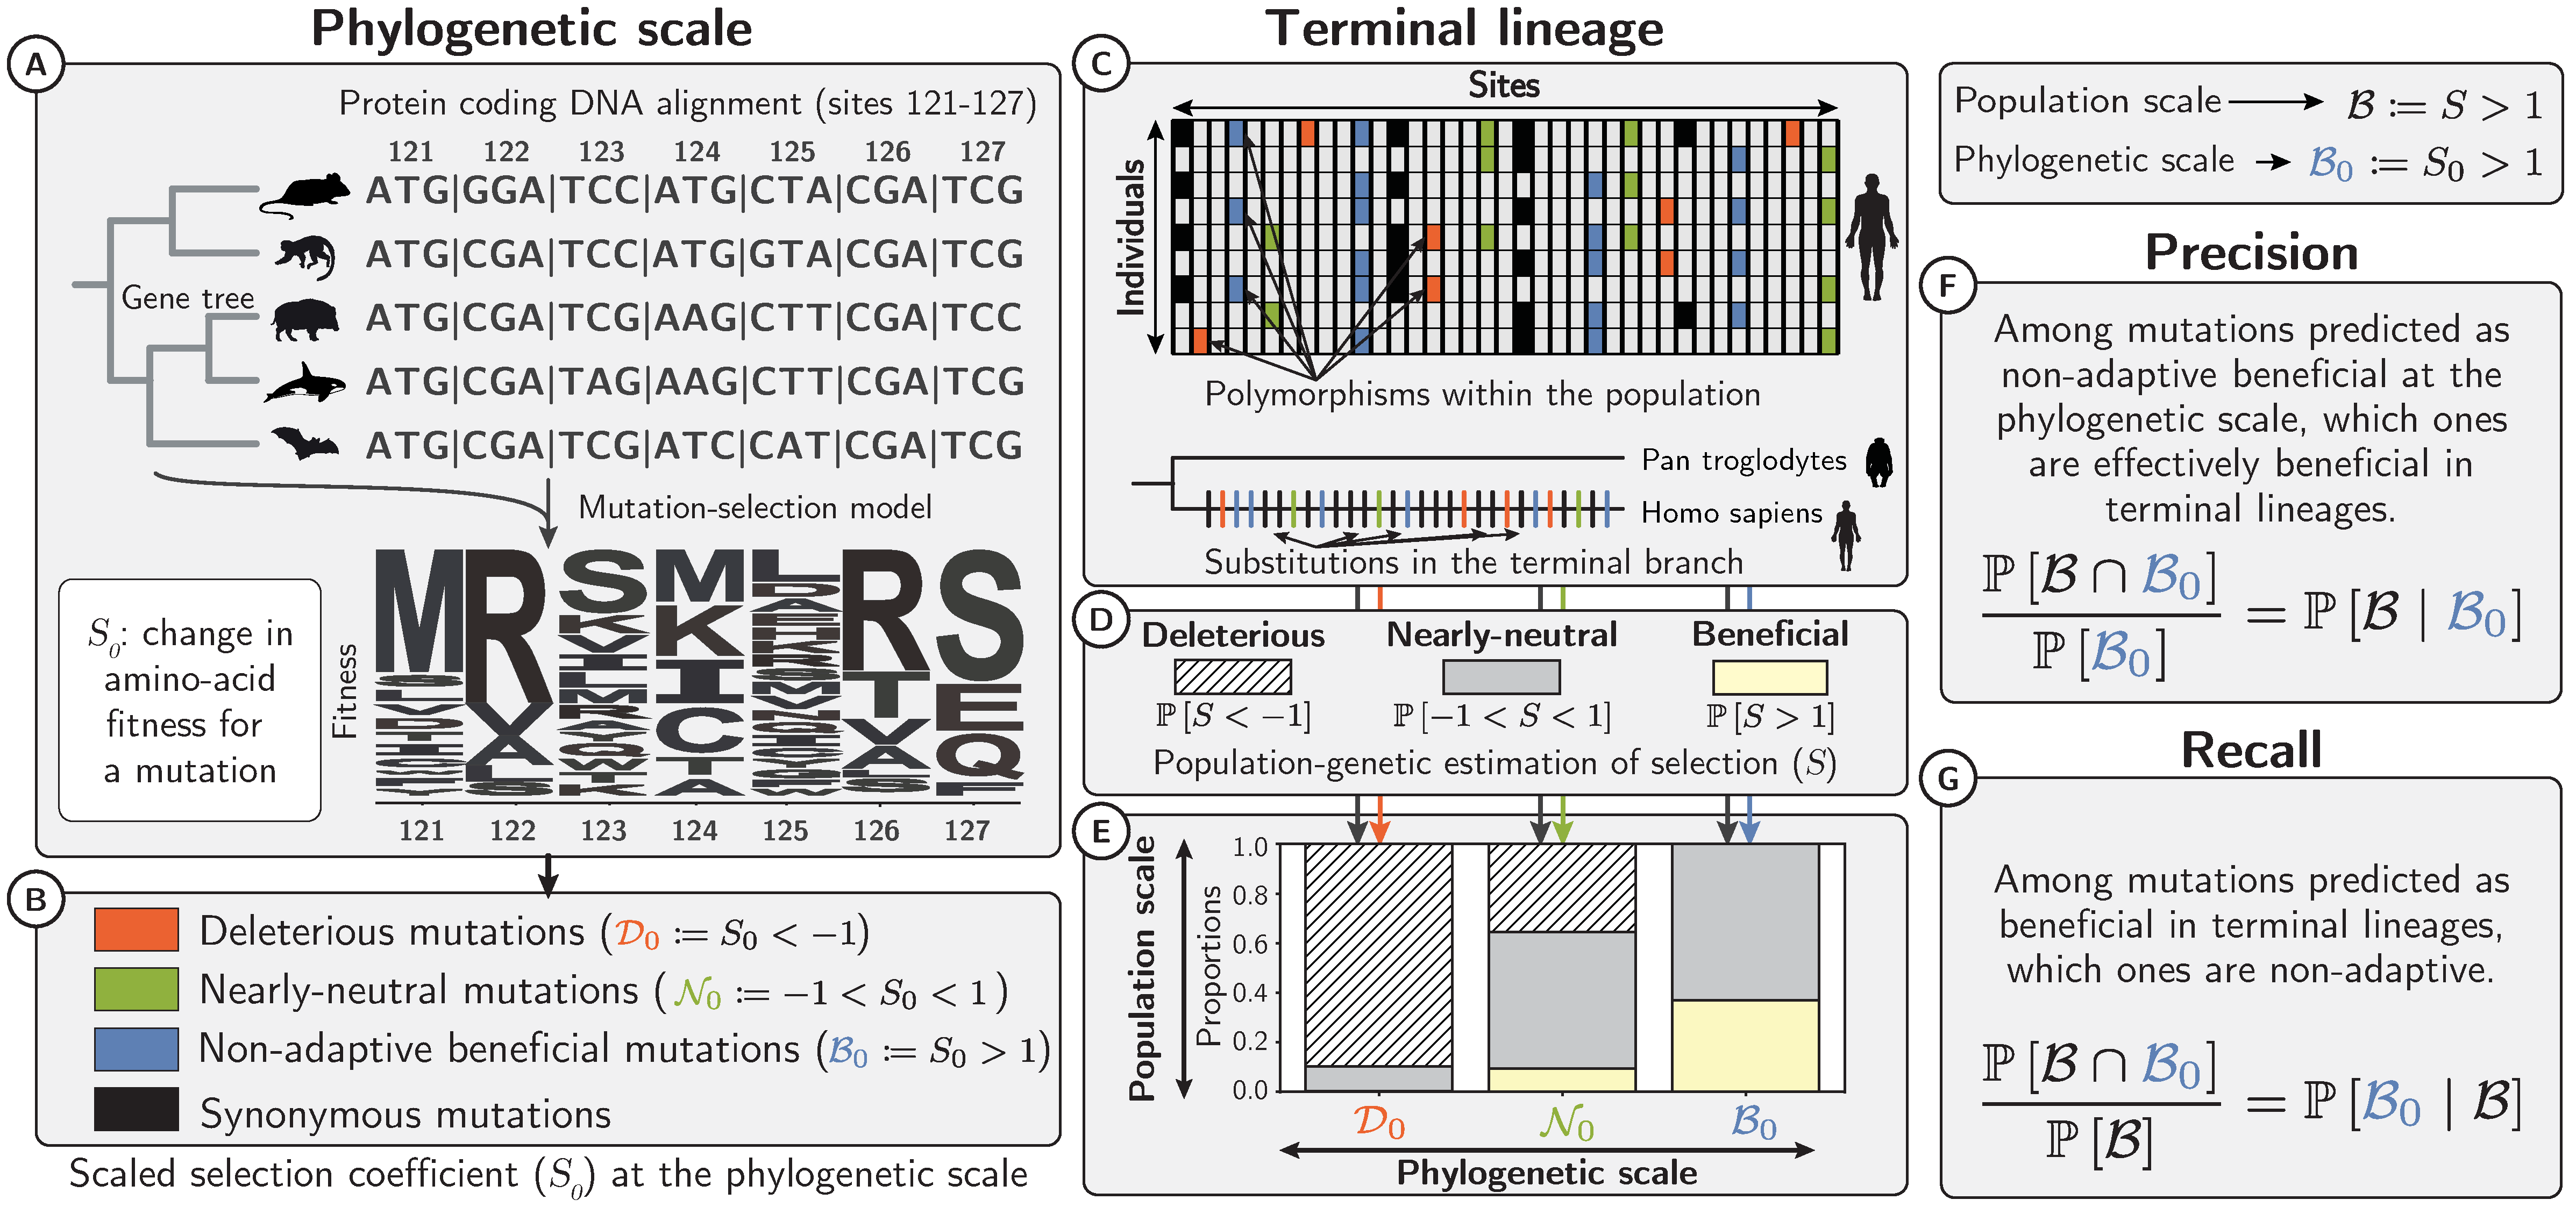
\includegraphics[width=\textwidth, page=1] {artworks/figure.method.proba.div.pdf}
            \captionof{figure}[Including substitutions in the terminal lineage to estimate $\Spop$]{\textbf{Including substitutions in the terminal lineage to estimate $\bm{\Spop}$.} Same as Figure 2 in the main text, but including substitutions in the terminal lineage to estimate $\Spop$.
            At the phylogenetic scale (A), we estimated the amino-acid fitness for each site from protein-coding DNA alignments using mutation-selection codon models.
            For every possible mutation, the difference in amino-acid fitness before and after the mutation allows us to compute the selection coefficient at the phylogenetic scale ($\Sphy$).
            Depending on $\Sphy$ (B) mutations can be predicted as deleterious ($\SphyDel$), nearly-neutral ($\SphyNeu$) or beneficial non-adaptive mutations ($\SphyBen$) toward a fitter amino acid and repairing existing functions.
            For each population, each observed single nucleotide polymorphism (SNP) segregating can also be classified according to its $\Sphy$ value (C).
            Within the terminal lineage leading to this population, each substitution can be classified according to its $\Spop$ value (C).
            Non-synonymous polymorphisms and divergence, contrasted to synonymous polymorphisms and divergence (deemed neutral) is used to estimate selection coefficients (D-E) at the population scale ($\Spop$), for each class of selection ($\SphyDel$, $\SphyNeu$, $\SphyBen$).
            We can thus assess whether $\Sphy$ predicts $\Spop$ and compute \textit{precision} (F) and \textit{recall} (G) for each class.
            The \textit{recall} value for class $\SphyBen$ is the probability for beneficial mutations to be non-adaptive (G).
            Icons are adapted from \href{https://phylopic.org}{https://phylopic.org} under a Creative Commons license.
            \label{fig-incdiv}
            }
    \end{center}

    \newpage

    \subsection{Probability for beneficial mutations to be non-adaptive}
    The estimation of $\proba{[} \SpopBen {]}$ and $\proba{[}\SphyBen\given \SpopBen {]}$ across populations when including substitutions in the terminal lineage and fitting a discrete DFE to $\Spop$ is shown in Table~\ref{table:inc-div-bayes}.
    Altogether, comparing these results with table~\ref{table:proba}, we acknowledge that the exact proportion of non-adaptive among all beneficial mutations is dependent whether we included or not substitutions in the terminal lineage for the estimation of $\Spop$.
    However, we can still see that non-adaptive beneficial mutations are positively selected compared to neutral and deleterious ones, and this result is valid whether we included or not substitutions in the terminal lineage for the estimation of $\Spop$.

    \begin{center}
        \scriptsize
        \begin{longtable*}{|l|l|r|r|r|r|r|r|}
            \toprule
            Population & Species & $\Ne$ & $\proba{[}\SphyBen{]}$ & $\proba{[} \SpopBen {]}$ & $\frac{\proba{[}\SphyBen]}{\proba{[} \SpopBen ]}$ & $\proba{[} \SpopBen \given \SphyBen{]}$ & $\proba{[}\SphyBen\given \SpopBen {]}$ \\
            \midrule
            \endhead
            \midrule
            \multicolumn{8}{r}{{Continued on next page}} \\
            \midrule
            \endfoot

            \bottomrule
            \endlastfoot
            \rowcolor{LIGHTGREY} Equus c. & Equus caballus & $7.5\times 10^{4}$ & $ 0.012$ & $ 0.057$ & $ 0.213$ & $ 0.498$ & $ 0.106$ \\
            Iran & Bos taurus & $5.6\times 10^{4}$ & $ 0.011$ & $ 0.006$ & $ 1.860$ & $ 0.368$ & $ 0.684$ \\
            Uganda & Bos taurus & $1.3\times 10^{5}$ & $ 0.011$ & $ 0.012$ & $ 0.900$ & $ 0.307$ & $ 0.276$ \\
            \rowcolor{LIGHTGREY} Australia & Capra hircus & $1.7\times 10^{5}$ & $ 0.011$ & $ 0.007$ & $ 1.651$ & $ 0.178$ & $ 0.294$ \\
            \rowcolor{LIGHTGREY} France & Capra hircus & $1.9\times 10^{5}$ & $ 0.011$ & $ 0.007$ & $ 1.614$ & $ 0.183$ & $ 0.295$ \\
            \rowcolor{LIGHTGREY} Iran (C. aegagrus) & Capra hircus & $1.9\times 10^{5}$ & $ 0.011$ & $ 0.012$ & $ 0.923$ & $ 0.177$ & $ 0.163$ \\
            \rowcolor{LIGHTGREY} Iran & Capra hircus & $2.3\times 10^{5}$ & $ 0.011$ & $ 0.008$ & $ 1.483$ & $ 0.184$ & $ 0.273$ \\
            \rowcolor{LIGHTGREY} Italy & Capra hircus & $1.9\times 10^{5}$ & $ 0.011$ & $ 0.007$ & $ 1.686$ & $ 0.178$ & $ 0.299$ \\
            \rowcolor{LIGHTGREY} Morocco & Capra hircus & $2.2\times 10^{5}$ & $ 0.011$ & $ 0.006$ & $ 1.892$ & $ 0.184$ & $ 0.349$ \\
            Iran & Ovis aries & $3.8\times 10^{5}$ & $ 0.012$ & $ 0.010$ & $ 1.132$ & $ 0.189$ & $ 0.214$ \\
            Iran (O. orientalis) & Ovis aries & $4.5\times 10^{5}$ & $ 0.011$ & $ 0.011$ & $ 1.012$ & $ 0.213$ & $ 0.216$ \\
            Iran (O. vignei) & Ovis aries & $3.7\times 10^{5}$ & $ 0.012$ & $ 0.021$ & $ 0.561$ & $ 0.186$ & $ 0.105$ \\
            Various & Ovis aries & $4.1\times 10^{5}$ & $ 0.011$ & $ 0.011$ & $ 1.069$ & $ 0.215$ & $ 0.229$ \\
            Morocco & Ovis aries & $ 4\times 10^{5}$ & $ 0.012$ & $ 0.012$ & $ 0.973$ & $ 0.217$ & $ 0.211$ \\
            \rowcolor{LIGHTGREY} Barbados & Chlorocebus sabaeus & $1.1\times 10^{5}$ & $ 0.009$ & $ 0.004$ & $ 2.120$ & $ 0.341$ & $ 0.723$ \\
            \rowcolor{LIGHTGREY} Central Afr. Rep. & Chlorocebus sabaeus & $1.7\times 10^{5}$ & $ 0.009$ & $ 0.013$ & $ 0.720$ & $ 0.368$ & $ 0.265$ \\
            \rowcolor{LIGHTGREY} Ethiopia & Chlorocebus sabaeus & $1.4\times 10^{5}$ & $ 0.009$ & $ 0.007$ & $ 1.352$ & $ 0.368$ & $ 0.498$ \\
            \rowcolor{LIGHTGREY} Gambia & Chlorocebus sabaeus & $1.4\times 10^{5}$ & $ 0.009$ & $ 0.010$ & $ 0.956$ & $ 0.368$ & $ 0.352$ \\
            \rowcolor{LIGHTGREY} Kenya & Chlorocebus sabaeus & $1.5\times 10^{5}$ & $ 0.009$ & $ 0.013$ & $ 0.727$ & $ 0.368$ & $ 0.268$ \\
            \rowcolor{LIGHTGREY} Nevis & Chlorocebus sabaeus & $ 1\times 10^{5}$ & $ 0.009$ & $ 0.004$ & $ 2.133$ & $ 0.368$ & $ 0.784$ \\
            \rowcolor{LIGHTGREY} South Africa & Chlorocebus sabaeus & $1.8\times 10^{5}$ & $ 0.009$ & $ 0.011$ & $ 0.874$ & $ 0.368$ & $ 0.322$ \\
            \rowcolor{LIGHTGREY} Saint Kitts & Chlorocebus sabaeus & $1.2\times 10^{5}$ & $ 0.009$ & $ 0.005$ & $ 1.905$ & $ 0.368$ & $ 0.701$ \\
            \rowcolor{LIGHTGREY} Zambia & Chlorocebus sabaeus & $1.7\times 10^{5}$ & $ 0.009$ & $ 0.014$ & $ 0.698$ & $ 0.368$ & $ 0.257$ \\
            African & Homo sapiens & $5.6\times 10^{4}$ & $ 0.010$ & $ 0.013$ & $ 0.726$ & $ 0.437$ & $ 0.317$ \\
            Admixed American & Homo sapiens & $4.5\times 10^{4}$ & $ 0.010$ & $ 0.011$ & $ 0.886$ & $ 0.429$ & $ 0.380$ \\
            East Asian & Homo sapiens & $ 4\times 10^{4}$ & $ 0.010$ & $ 0.008$ & $ 1.213$ & $ 0.426$ & $ 0.517$ \\
            European & Homo sapiens & $4.1\times 10^{4}$ & $ 0.010$ & $ 0.009$ & $ 1.104$ & $ 0.422$ & $ 0.466$ \\
            South Asian & Homo sapiens & $4.4\times 10^{4}$ & $ 0.010$ & $ 0.009$ & $ 1.016$ & $ 0.426$ & $ 0.433$ \\
        \end{longtable*}
        \captionof{table}[$\proba{[}\SphyBen\given \SpopBen {]}$ when including divergence to estimate $\Spop$.]{\textbf{$\bm{\proba{[}\SphyBen\given \SpopBen {]}}$ when including divergence to estimate $\bm{\Spop}$.}
        $\Ne$ is the estimated effective population size.
        $\proba{[} \SphyBen {]}$ (eq.~5) is the probability for a new mutation to be a non-adaptive mutation.
        These mutations have a selection coefficient predicted at the phylogenetic-scale larger than 1, thus toward a more fit amino-acid.
        $\proba{[} \SpopBen {]}$ (eq.~15) is the probability for a mutation to be beneficial.
        These mutations have a selection coefficient at the population-scale larger than 1.
        $\proba{[} \SpopBen \given \SphyBen{]}$ (eq.~12) is the probability for a mutation to be beneficial at the population scale, given it is predicted to be a non-adaptive mutation at the phylogenetic scale (the \textit{precision}).
        $\proba{[} \SphyBen \given \SpopBen{]}$ (eq.~14) is the probability for a mutation to be non-adaptive given it is beneficial at the population scale (the \textit{recall}).
        This probability is obtained using Bayes' formula.\label{table:inc-div-bayes}}
    \end{center}

    \newpage

    \subsection{Precision and recall}
    The estimation of \textit{precision} and \textit{recall} across populations when including substitutions in the terminal lineage for the estimation of $\Spop$ is shown in Table~\ref{table:inc-div}.
    Comparing these results with tables 1, we acknowledge that the exact quantification of \textit{precision} and \textit{recall} is dependent on whether we included or not substitutions in the terminal lineage for the estimation of $\Spop$.
    However, we can still see that non-adaptive beneficial mutations are positively selected compared to neutral and deleterious ones, and this result is valid whether we included or not substitutions in the terminal lineage for the estimation of $\Spop$.

    \begin{center}
        \begin{adjustbox}{width=\textwidth}
            \begin{tabular}{||l|l|r||r|r||r|r||r|r||}
                \toprule
                \multicolumn{3}{||c||}{} &
                \multicolumn{2}{c||}{\shortstack{\textbf{Deleterious mutations} \\ $\bm{\SpopDel \coloneqq \Spop<-1}$ \\ $\bm{\SphyDel \coloneqq \Sphy<-1}$}} &
                \multicolumn{2}{c||}{\shortstack{\textbf{Nearly-neutral mutations} \\ $\bm{\SpopNeu \coloneqq -1<\Spop<1}$ \\ $\bm{\SphyNeu \coloneqq -1<\Sphy<1}$}} &
                \multicolumn{2}{c||}{\shortstack{\textbf{Beneficial mutations} \\ $\bm{\SpopBen \coloneqq \Spop>1}$ \\ $\bm{\SphyBen \coloneqq \Sphy>1}$}}
                \\ \hline
                \textbf{Population} &
                \textbf{Species} &
                $\bm{\Ne}$ &
                \makecell{\textbf{Precision} \\ $\bm{\proba{[}\SpopDel \given \SphyDel]}$} &
                \makecell{\textbf{Recall} \\ $\bm{\proba{[}\SphyDel \given \SpopDel]}$}           &
                \makecell{\textbf{Precision}      \\ $\bm{\proba{[}\SpopNeu \given \SphyNeu]}$}                                    &
                \makecell{\textbf{Recall}          \\ $\bm{\proba{[}\SphyNeu \given \SpopNeu]}$}                                  &
                \makecell{\textbf{Precision}          \\ $\bm{\proba{[}\SpopBen \given \SphyBen]}$}          &
                \makecell{\textbf{Recall}        \\ $\bm{\proba{[}\SphyBen \given \SpopBen]}$}
                \\   \midrule
                \rowcolor{LIGHTGREY} Equus c. & Equus caballus & $7.5\times 10^{4}$ & $ 0.937$ & $ 0.955$ & $ 0.111$ & $ 0.192$ & $ 0.498$ & $ 0.106$ \\
                Iran & Bos taurus & $5.6\times 10^{4}$ & $ 0.935$ & $ 0.970$ & $ 0.565$ & $ 0.356$ & $ 0.368$ & $ 0.684$ \\
                Uganda & Bos taurus & $1.3\times 10^{5}$ & $ 0.951$ & $ 0.967$ & $ 0.516$ & $ 0.422$ & $ 0.307$ & $ 0.276$ \\
                \rowcolor{LIGHTGREY} Australia & Capra hircus & $1.7\times 10^{5}$ & $ 0.952$ & $ 0.970$ & $ 0.598$ & $ 0.452$ & $ 0.178$ & $ 0.294$ \\
                \rowcolor{LIGHTGREY} France & Capra hircus & $1.9\times 10^{5}$ & $ 0.951$ & $ 0.969$ & $ 0.574$ & $ 0.433$ & $ 0.183$ & $ 0.295$ \\
                \rowcolor{LIGHTGREY} Iran (C. aegagrus) & Capra hircus & $1.9\times 10^{5}$ & $ 0.957$ & $ 0.966$ & $ 0.515$ & $ 0.460$ & $ 0.177$ & $ 0.163$ \\
                \rowcolor{LIGHTGREY} Iran & Capra hircus & $2.3\times 10^{5}$ & $ 0.951$ & $ 0.967$ & $ 0.542$ & $ 0.422$ & $ 0.184$ & $ 0.273$ \\
                \rowcolor{LIGHTGREY} Italy & Capra hircus & $1.9\times 10^{5}$ & $ 0.951$ & $ 0.969$ & $ 0.582$ & $ 0.436$ & $ 0.178$ & $ 0.299$ \\
                \rowcolor{LIGHTGREY} Morocco & Capra hircus & $2.2\times 10^{5}$ & $ 0.949$ & $ 0.968$ & $ 0.556$ & $ 0.412$ & $ 0.184$ & $ 0.349$ \\
                Iran & Ovis aries & $3.8\times 10^{5}$ & $ 0.963$ & $ 0.962$ & $ 0.421$ & $ 0.424$ & $ 0.189$ & $ 0.214$ \\
                Iran (O. orientalis) & Ovis aries & $4.5\times 10^{5}$ & $ 0.968$ & $ 0.961$ & $ 0.413$ & $ 0.460$ & $ 0.213$ & $ 0.216$ \\
                Iran (O. vignei) & Ovis aries & $3.7\times 10^{5}$ & $ 0.972$ & $ 0.959$ & $ 0.360$ & $ 0.528$ & $ 0.186$ & $ 0.105$ \\
                Various & Ovis aries & $4.1\times 10^{5}$ & $ 0.966$ & $ 0.961$ & $ 0.430$ & $ 0.454$ & $ 0.215$ & $ 0.229$ \\
                Morocco & Ovis aries & $ 4\times 10^{5}$ & $ 0.966$ & $ 0.958$ & $ 0.372$ & $ 0.416$ & $ 0.217$ & $ 0.211$ \\
                \rowcolor{LIGHTGREY} Barbados & Chlorocebus sabaeus & $1.1\times 10^{5}$ & $ 0.940$ & $ 0.976$ & $ 0.654$ & $ 0.409$ & $ 0.341$ & $ 0.723$ \\
                \rowcolor{LIGHTGREY} Central Afr. Rep. & Chlorocebus sabaeus & $1.7\times 10^{5}$ & $ 0.950$ & $ 0.971$ & $ 0.526$ & $ 0.421$ & $ 0.368$ & $ 0.265$ \\
                \rowcolor{LIGHTGREY} Ethiopia & Chlorocebus sabaeus & $1.4\times 10^{5}$ & $ 0.942$ & $ 0.974$ & $ 0.609$ & $ 0.402$ & $ 0.368$ & $ 0.498$ \\
                \rowcolor{LIGHTGREY} Gambia & Chlorocebus sabaeus & $1.4\times 10^{5}$ & $ 0.950$ & $ 0.974$ & $ 0.611$ & $ 0.452$ & $ 0.368$ & $ 0.352$ \\
                \rowcolor{LIGHTGREY} Kenya & Chlorocebus sabaeus & $1.5\times 10^{5}$ & $ 0.950$ & $ 0.972$ & $ 0.545$ & $ 0.434$ & $ 0.368$ & $ 0.268$ \\
                \rowcolor{LIGHTGREY} Nevis & Chlorocebus sabaeus & $ 1\times 10^{5}$ & $ 0.940$ & $ 0.977$ & $ 0.668$ & $ 0.412$ & $ 0.368$ & $ 0.784$ \\
                \rowcolor{LIGHTGREY} South Africa & Chlorocebus sabaeus & $1.8\times 10^{5}$ & $ 0.947$ & $ 0.972$ & $ 0.550$ & $ 0.411$ & $ 0.368$ & $ 0.322$ \\
                \rowcolor{LIGHTGREY} Saint Kitts & Chlorocebus sabaeus & $1.2\times 10^{5}$ & $ 0.940$ & $ 0.976$ & $ 0.646$ & $ 0.407$ & $ 0.368$ & $ 0.701$ \\
                \rowcolor{LIGHTGREY} Zambia & Chlorocebus sabaeus & $1.7\times 10^{5}$ & $ 0.950$ & $ 0.971$ & $ 0.527$ & $ 0.426$ & $ 0.368$ & $ 0.257$ \\
                African & Homo sapiens & $5.6\times 10^{4}$ & $ 0.911$ & $ 0.980$ & $ 0.666$ & $ 0.341$ & $ 0.437$ & $ 0.317$ \\
                Admixed American & Homo sapiens & $4.5\times 10^{4}$ & $ 0.902$ & $ 0.976$ & $ 0.580$ & $ 0.284$ & $ 0.429$ & $ 0.380$ \\
                East Asian & Homo sapiens & $ 4\times 10^{4}$ & $ 0.904$ & $ 0.984$ & $ 0.744$ & $ 0.341$ & $ 0.426$ & $ 0.517$ \\
                European & Homo sapiens & $4.1\times 10^{4}$ & $ 0.906$ & $ 0.984$ & $ 0.737$ & $ 0.344$ & $ 0.422$ & $ 0.466$ \\
                South Asian & Homo sapiens & $4.4\times 10^{4}$ & $ 0.907$ & $ 0.984$ & $ 0.737$ & $ 0.349$ & $ 0.426$ & $ 0.433$ \\
                \bottomrule
            \end{tabular}
        \end{adjustbox}
        \captionof{table}[Precision and recall when including divergence to estimate $\Spop$.]{\textbf{Precision and recall when including divergence to estimate $\bm{\Spop}$.}
        $\Ne$ is the estimated effective population size.
        \textit{Precision} is the estimation of the selection coefficient at population scale ($\Spop$) given that $\Sphy$ is known.
        \textit{Recall} is the estimation of $\Sphy$ given selection coefficient at the population scale ($\Spop$) is known.
        \textit{Recall} for beneficial mutations ($\proba{[}\SphyBen \given \SpopBen{]}$) is the probability for a mutation to be non-adaptive given it is beneficial at the population scale.
        \label{table:inc-div}}
    \end{center}

    \newpage

    \subsection{Misannotations of ancestral alleles}

    If misannotation is influencing the recall for $\SphyBen$ ($\proba{[}\SphyBen\given \SpopBen {]}$), then the recall should increase as a function of  divergence to the sister species ($\ds$: number of synonymous substitutions per sites) since divergence would increase the rate of misannotations.
    Shown in Figure~\ref{fig:distance-incdiv} is recall $\proba{[}\SphyBen\given \SpopBen {]}$ as a function of divergence ($\ds$) in which the latter is not an explanatory variable.

    \begin{center}
        \includegraphics[width=0.75\linewidth, page=1]{artworks/results.distance.recall_pos.div.scatter.pdf}
        \captionof{figure}[$\proba{[}\SphyBen\given \SpopBen {]}$ when including divergence to estimate $\Spop$, as a function of distance to the sister species.]{\textbf{$\bm{\proba{[}\SphyBen\given \SpopBen {]}}$ when including divergence to estimate $\bm{\Spop}$, as a function of distance to the sister species}. $\proba{[} \SphyBen \given \SpopBen{]}$ (eq.~14) is the probability for a beneficial mutation to be non-adaptive. $\ds$ is number of synonymous substitutions per site that occurred since divergence with the sister species (closest species in the mammalian tree). Same as Figure~\ref{fig:distance-sister} but including divergence to estimate $\Spop$. Populations are represented by circles, and squares are the mean for the species. Correlations account for phylogenetic relationship and non-independence of samples, through the fit of a Phylogenetic Generalized Linear Model (see Materials \& Methods).\label{fig:distance-incdiv}}
    \end{center}

    \newpage

    \subsection{Excluding genes under adaptation}
    The proportion of beneficial non-adaptive mutations ($\proba{[}\SphyBen\given \SpopBen {]}$) is higher when excluding genes under adaptation, as shown in Table~\ref{table:no-adaptation-div}, consistent with our expectation that genes with uniformly conserved functions should fit better the nearly-neutral equilibrium model.

    \begin{center}
        \begin{tabular}{|l|l|r|r|}
            \toprule
            Population & Species & Control & Case \\
            \midrule
            \rowcolor{LIGHTGREY} Equus c. & Equus caballus & $ 0.106$ & $ 0.106$ \\
            Iran & Bos taurus & $ 0.684$ & $ 0.755$ \\
            Uganda & Bos taurus & $ 0.276$ & $ 0.310$ \\
            \rowcolor{LIGHTGREY} Australia & Capra hircus & $ 0.294$ & $ 0.319$ \\
            \rowcolor{LIGHTGREY} France & Capra hircus & $ 0.295$ & $ 0.325$ \\
            \rowcolor{LIGHTGREY} Iran (C. aegagrus) & Capra hircus & $ 0.163$ & $ 0.174$ \\
            \rowcolor{LIGHTGREY} Iran & Capra hircus & $ 0.273$ & $ 0.299$ \\
            \rowcolor{LIGHTGREY} Italy & Capra hircus & $ 0.299$ & $ 0.321$ \\
            \rowcolor{LIGHTGREY} Morocco & Capra hircus & $ 0.349$ & $ 0.419$ \\
            Iran & Ovis aries & $ 0.214$ & $ 0.241$ \\
            Iran (O. orientalis) & Ovis aries & $ 0.216$ & $ 0.213$ \\
            Iran (O. vignei) & Ovis aries & $ 0.105$ & $ 0.089$ \\
            Various & Ovis aries & $ 0.229$ & $ 0.196$ \\
            Morocco & Ovis aries & $ 0.211$ & $ 0.206$ \\
            \rowcolor{LIGHTGREY} Barbados & Chlorocebus sabaeus & $ 0.723$ & $ 0.833$ \\
            \rowcolor{LIGHTGREY} Central Afr. Rep. & Chlorocebus sabaeus & $ 0.265$ & $ 0.285$ \\
            \rowcolor{LIGHTGREY} Ethiopia & Chlorocebus sabaeus & $ 0.498$ & $ 0.547$ \\
            \rowcolor{LIGHTGREY} Gambia & Chlorocebus sabaeus & $ 0.352$ & $ 0.571$ \\
            \rowcolor{LIGHTGREY} Kenya & Chlorocebus sabaeus & $ 0.268$ & $ 0.265$ \\
            \rowcolor{LIGHTGREY} Nevis & Chlorocebus sabaeus & $ 0.784$ & $ 0.892$ \\
            \rowcolor{LIGHTGREY} South Africa & Chlorocebus sabaeus & $ 0.322$ & $ 0.307$ \\
            \rowcolor{LIGHTGREY} Saint Kitts & Chlorocebus sabaeus & $ 0.701$ & $ 0.825$ \\
            \rowcolor{LIGHTGREY} Zambia & Chlorocebus sabaeus & $ 0.257$ & $ 0.271$ \\
            African & Homo sapiens & $ 0.317$ & $ 0.278$ \\
            Admixed American & Homo sapiens & $ 0.380$ & $ 0.363$ \\
            East Asian & Homo sapiens & $ 0.517$ & $ 0.499$ \\
            European & Homo sapiens & $ 0.466$ & $ 0.456$ \\
            South Asian & Homo sapiens & $ 0.433$ & $ 0.304$ \\
            \bottomrule
        \end{tabular}
        \captionof{table}[$\proba{[}\SphyBen\given \SpopBen {]}$ excluding or not genes under adaptation, when including divergence to estimate $\Spop$.]{\textbf{$\bm{\proba{[}\SphyBen\given \SpopBen {]}}$ excluding or not genes under adaptation, when including divergence to estimate $\bm{\Spop}$.}
        Genes under adaptation retrieved from~\cite{latrille_genes_2023}.
        Comparison of $\proba{[}\SphyBen\given \SpopBen {]}$ when including divergence for the whole genome (control) and when excluding genes under adaptation (case).
        The non-parametric Wilcoxon signed-rank test tests the null hypothesis that the distribution of the differences (case versus control) is symmetric about zero.
        Applied to the paired samples (case and control), Wilcoxon signed-rank test results in $s=120$ with $\pvalue=0.027$ for one-sided test (case higher than control).\label{table:no-adaptation-div}
        }
    \end{center}


    \newpage
    \subsection{Fitting one or three distributions of fitness effects}

    We also performed another test to assess that fitting the same functional form of DFE to three categories of selection (i.e., $\SphyDel, \SphyNeu, \SphyBen$) is a sound methodology.
    Typically, $\proba{[} \SpopBen {]}$ can be computed from two different estimates, by either splitting data (polymorphism within populations and substitutions in the terminal lineages) in three category (i.e., $\SphyDel, \SphyNeu, \SphyBen$) or not at all.
    In the case of splitting data in three categories and fitting three DFEs, $\proba{[} \SpopBen {]}$ is obtained by summing over the three categories using the law of total probability (eq.\ 15):

    \begin{equation}
        \proba{[} \SpopBen ] \text{ (three DFEs) } = \proba{[}\SpopBen \given \SphyDel ] \times \proba{[}\SphyDel ] + \proba{[}\SpopBen \given \SphyNeu ] \times \proba{[}\SphyNeu ] + \proba{[}\SpopBen \given \SphyBen ] \times \proba{[}\SphyBen ].
        \label{eq:total_proba}
    \end{equation}

    But it is also possible to compute $\proba{[} \SpopBen {]}$ directly from fitting one DFE to the full data (polymorphism within populations and substitutions in the terminal lineages), not splitting at all, and then $\proba{[} \SpopBen {]}$ is obtained from the parameters of the DFE (eq.\ 11):
    \begin{align}
        \proba{[} \SpopBen ] \text{ (one DFE) } &= \proba{[} \Spop > 1 ] = p_b \int_{1}^{+\infty} f_{e}(\Spop; \AdvMean) \der \Spop. \label{eq:polyProbaAdv}
    \end{align}

    We reproduced this experiment for $\proba{[} \SpopDel {]}$ (Figure~\ref{fig:one-three-neg}), $\proba{[} \SpopNeu {]}$ (Figure~\ref{fig:one-three-weak}) and $\proba{[} \SpopBen {]}$ (Figure~\ref{fig:one-three-pos}).


    \begin{center}
        \includegraphics[width=0.75\linewidth, page=1]{artworks/results.reg.neg.div.scatter.pdf}
        \captionof{figure}[$\proba{[} \SpopDel {]}$ when fitting a single or three DFEs.]{\textbf{$\bm{\proba{[} \SpopDel {]}}$ when fitting a single or three DFEs.} Populations are represented by circles, and squares are the mean for the species. Goodness of fit is calculated as the coefficient of determination ($R^2$) for the prediction $\proba{[} \SpopDel ] \text{ (three DFEs) } = \proba{[} \SpopDel ] \text{ (one DFE) }$, meaning calculating the residuals of the fit to the 1:1 line.\label{fig:one-three-neg}}
    \end{center}

    \newpage
    \begin{center}
        \includegraphics[width=0.75\linewidth, page=1]{artworks/results.reg.weak.div.scatter.pdf}
        \captionof{figure}[$\proba{[} \SpopNeu {]}$ when fitting a single or three DFEs.]{\textbf{$\bm{\proba{[} \SpopNeu {]}}$ when fitting a single or three DFEs.} Populations are represented by circles, and squares are the mean for the species. Goodness of fit is calculated as the coefficient of determination ($R^2$) for the prediction $\proba{[} \SpopNeu ] \text{ (three DFEs) } = \proba{[} \SpopNeu ] \text{ (one DFE) }$, meaning calculating the residuals of the fit to the 1:1 line.\label{fig:one-three-weak}}
    \end{center}

    \begin{center}
        \includegraphics[width=0.75\linewidth, page=1]{artworks/results.reg.pos.div.scatter.pdf}
        \captionof{figure}[$\proba{[} \SpopBen {]}$ when fitting a single or three DFEs.]{\textbf{$\bm{\proba{[} \SpopBen {]}}$ when fitting a single or three DFEs.} Populations are represented by circles, and squares are the mean for the species. Goodness of fit is calculated as the coefficient of determination ($R^2$) for the prediction $\proba{[} \SpopBen ] \text{ (three DFEs) } = \proba{[} \SpopBen ] \text{ (one DFE) }$, meaning calculating the residuals of the fit to the 1:1 line.\label{fig:one-three-pos}}
    \end{center}

    \newpage

    \section{Non-parametric distribution of fitness effects}

    \subsection{polyDFE model D (non-parametric)}
    Additionally to including divergence, we also tested our prediction with polyDFE model D instead of model C.
    In polyDFE model D, the DFE of non-synonymous mutations is given as a discrete DFE of $K$ categories (instead of a continuous distribution in model C), where the selection coefficients of each category $i$ ($1 \leq i \leq K$) are fixed parameters $\Spop_i$, and each value $\Spop_i$ has a probability $p_i$ (estimated), with $\sum_{i=1}^{K} p_i =1$.
    We used $K=6$ with $\Spop_1 = -500$, $\Spop_2 = -4$, $\Spop_3 =-1$, $\Spop_4 = 0$, $\Spop_5 = 1$, $\Spop_6 = 4$.\\

    For each class of selection $\Sphyclass$, the parameters $p_i$ ($i \in \{ 1 \leq i \leq 6 \}$) were used to compute $\proba{[} \SpopDel \given  \Sphyclass{]}$, $\proba{[} \SpopNeu \given \Sphyclass{]}$, and $\proba{[} \SpopBen \given \Sphyclass{]}$ as:
    \begin{align}
        \proba{[} \SpopDel \given  \Sphyclass] &= \proba{[} \Spop < -1 \given \Sphyclass ] = p_1 + p_2 \label{eq:polyProbaDel-mD} \\
        \proba{[} \SpopNeu \given \Sphyclass] &= \proba{[} -1 < \Spop < 1 \given \Sphyclass ] = p_3 + p_4 + p_5,  \\
        \proba{[} \SpopBen \given \Sphyclass] &= \proba{[}  \Spop > 1 \given \Sphyclass ] = p_6.  \label{eq:polyProbaAdv-mD}
    \end{align}

    \newpage
    \subsection{Probability for beneficial mutations to be non-adaptive}
    The estimation of $\proba{[} \SpopBen {]}$ and $\proba{[}\SphyBen\given \SpopBen {]}$ across populations when including substitutions in the terminal lineage and fitting a discrete DFE to $\Spop$ is shown in Table~\ref{table:discrete-dfe-bayes}.
    Altogether, comparing these results with table~\ref{table:inc-div-bayes}, we acknowledge that the exact proportion of non-adaptive among all beneficial mutations is dependent on the model used to estimate the DFE.
    However, we can still see that non-adaptive beneficial mutations are positively selected compared to neutral and deleterious ones, and this result is valid for different underlying DFE.

    \begin{center}
        \scriptsize
        \begin{longtable*}{|l|l|r|r|r|r|r|r|}
            \toprule
            Population & Species & $\Ne$ & $\proba{[}\SphyBen{]}$ & $\proba{[} \SpopBen {]}$ & $\frac{\proba{[}\SphyBen]}{\proba{[} \SpopBen ]}$ & $\proba{[} \SpopBen \given \SphyBen{]}$ & $\proba{[}\SphyBen\given \SpopBen {]}$ \\
            \midrule
            \endhead
            \midrule
            \multicolumn{8}{r}{{Continued on next page}} \\
            \midrule
            \endfoot

            \bottomrule
            \endlastfoot
            \rowcolor{LIGHTGREY} Equus c. & Equus caballus & $7.5\times 10^{4}$ & $ 0.012$ & $ 0.006$ & $ 2.050$ & $ 0.163$ & $ 0.334$ \\
            Iran & Bos taurus & $5.6\times 10^{4}$ & $ 0.011$ & $ 0.005$ & $ 2.125$ & $ 0.133$ & $ 0.283$ \\
            Uganda & Bos taurus & $1.3\times 10^{5}$ & $ 0.011$ & $ 0.010$ & $ 1.139$ & $ 0.140$ & $ 0.159$ \\
            \rowcolor{LIGHTGREY} Australia & Capra hircus & $1.7\times 10^{5}$ & $ 0.011$ & $ 0.002$ & $ 5.637$ & $ 0.151$ & $ 0.850$ \\
            \rowcolor{LIGHTGREY} France & Capra hircus & $1.9\times 10^{5}$ & $ 0.011$ & $ 0.002$ & $ 6.117$ & $ 0.154$ & $ 0.940$ \\
            \rowcolor{LIGHTGREY} Iran (C. aegagrus) & Capra hircus & $1.9\times 10^{5}$ & $ 0.011$ & $ 0.002$ & $ 5.842$ & $ 0.156$ & $ 0.911$ \\
            \rowcolor{LIGHTGREY} Iran & Capra hircus & $2.3\times 10^{5}$ & $ 0.011$ & $ 0.002$ & $ 6.400$ & $ 0.147$ & $ 0.943$ \\
            \rowcolor{LIGHTGREY} Italy & Capra hircus & $1.9\times 10^{5}$ & $ 0.011$ & $ 0.002$ & $ 5.793$ & $ 0.155$ & $ 0.895$ \\
            \rowcolor{LIGHTGREY} Morocco & Capra hircus & $2.2\times 10^{5}$ & $ 0.011$ & $ 0.003$ & $ 4.192$ & $ 0.150$ & $ 0.627$ \\
            Iran & Ovis aries & $3.8\times 10^{5}$ & $ 0.012$ & $ 0.020$ & $ 0.584$ & $ 0.154$ & $ 0.090$ \\
            Iran (O. orientalis) & Ovis aries & $4.5\times 10^{5}$ & $ 0.011$ & $ 0.021$ & $ 0.535$ & $ 0.148$ & $ 0.079$ \\
            Iran (O. vignei) & Ovis aries & $3.7\times 10^{5}$ & $ 0.012$ & $ 0.020$ & $ 0.568$ & $ 0.151$ & $ 0.086$ \\
            Various & Ovis aries & $4.1\times 10^{5}$ & $ 0.011$ & $ 0.021$ & $ 0.553$ & $ 0.152$ & $ 0.084$ \\
            Morocco & Ovis aries & $ 4\times 10^{5}$ & $ 0.012$ & $ 0.022$ & $ 0.529$ & $ 0.153$ & $ 0.081$ \\
            \rowcolor{LIGHTGREY} Barbados & Chlorocebus sabaeus & $1.1\times 10^{5}$ & $ 0.009$ & $ 0.002$ & $ 5.152$ & $ 0.170$ & $ 0.877$ \\
            \rowcolor{LIGHTGREY} Central Afr. Rep. & Chlorocebus sabaeus & $1.7\times 10^{5}$ & $ 0.009$ & $ 0.007$ & $ 1.266$ & $ 0.157$ & $ 0.199$ \\
            \rowcolor{LIGHTGREY} Ethiopia & Chlorocebus sabaeus & $1.4\times 10^{5}$ & $ 0.009$ & $ 0.002$ & $ 3.979$ & $ 0.161$ & $ 0.640$ \\
            \rowcolor{LIGHTGREY} Gambia & Chlorocebus sabaeus & $1.4\times 10^{5}$ & $ 0.009$ & $ 0.008$ & $ 1.201$ & $ 0.159$ & $ 0.191$ \\
            \rowcolor{LIGHTGREY} Kenya & Chlorocebus sabaeus & $1.5\times 10^{5}$ & $ 0.009$ & $ 0.003$ & $ 2.801$ & $ 0.165$ & $ 0.461$ \\
            \rowcolor{LIGHTGREY} Nevis & Chlorocebus sabaeus & $ 1\times 10^{5}$ & $ 0.009$ & $ 0.002$ & $ 5.361$ & $ 0.169$ & $ 0.908$ \\
            \rowcolor{LIGHTGREY} South Africa & Chlorocebus sabaeus & $1.8\times 10^{5}$ & $ 0.009$ & $ 0.005$ & $ 1.912$ & $ 0.154$ & $ 0.294$ \\
            \rowcolor{LIGHTGREY} Saint Kitts & Chlorocebus sabaeus & $1.2\times 10^{5}$ & $ 0.009$ & $ 0.002$ & $ 4.561$ & $ 0.165$ & $ 0.753$ \\
            \rowcolor{LIGHTGREY} Zambia & Chlorocebus sabaeus & $1.7\times 10^{5}$ & $ 0.009$ & $ 0.004$ & $ 2.661$ & $ 0.153$ & $ 0.406$ \\
            African & Homo sapiens & $5.6\times 10^{4}$ & $ 0.010$ & $ 0.010$ & $ 0.997$ & $ 0.154$ & $ 0.154$ \\
            Admixed American & Homo sapiens & $4.5\times 10^{4}$ & $ 0.010$ & $ 0.008$ & $ 1.206$ & $ 0.158$ & $ 0.190$ \\
            East Asian & Homo sapiens & $ 4\times 10^{4}$ & $ 0.010$ & $ 0.007$ & $ 1.455$ & $ 0.163$ & $ 0.237$ \\
            European & Homo sapiens & $4.2\times 10^{4}$ & $ 0.010$ & $ 0.007$ & $ 1.316$ & $ 0.167$ & $ 0.219$ \\
            South Asian & Homo sapiens & $4.4\times 10^{4}$ & $ 0.010$ & $ 0.007$ & $ 1.340$ & $ 0.164$ & $ 0.219$ \\
        \end{longtable*}
        \captionof{table}[$\proba{[}\SphyBen\given \SpopBen {]}$ when using a discrete DFE to estimate $\Spop$.]{\textbf{$\bm{\proba{[}\SphyBen\given \SpopBen {]}}$ when using a discrete DFE to estimate $\bm{\Spop}$.}
        $\Ne$ is the estimated effective population size.
        $\proba{[} \SphyBen {]}$ (eq.~5) is the probability for a new mutation to be a non-adaptive beneficial mutation.
        These mutations have a selection coefficient predicted at the phylogenetic-scale larger than 1, thus toward a more fit amino-acid.
        $\proba{[} \SpopBen {]}$ (eq.~15) is the probability for a mutation to be beneficial.
        These mutations have a selection coefficient at the population-scale larger than 1.
        $\proba{[} \SpopBen \given \SphyBen{]}$ (eq.~12) is the probability for a mutation to be beneficial at the population scale, given it is predicted to be a beneficial non-adaptive mutation at the phylogenetic scale (the \textit{precision}).
        $\proba{[} \SphyBen \given \SpopBen{]}$ (eq.~14) is the probability for a mutation to be non-adaptive given it is beneficial at the population scale (the \textit{recall}).
        This probability is obtained using Bayes' formula.\label{table:discrete-dfe-bayes}}
    \end{center}

    \newpage
    \subsection{Precision and recall}
    The estimation of \textit{precision} and \textit{recall} across populations when including substitutions in the terminal lineage and fitting a discrete DFE to $\Spop$ is shown in Table~\ref{table:discrete-dfe}.
    Altogether, comparing these results with table~\ref{table:inc-div}, we acknowledge that the exact quantification of \textit{precision} and \textit{recall} is dependent on the model used to estimate the DFE.
    However, we can still see that non-adaptive beneficial mutations are positively selected compared to neutral and deleterious ones, and this result is valid for different underlying DFE.

    \begin{center}
        \begin{adjustbox}{width=\textwidth}
            \begin{tabular}{||l|l|r||r|r||r|r||r|r||}
                \toprule
                \multicolumn{3}{||c||}{} &
                \multicolumn{2}{c||}{\shortstack{\textbf{Deleterious mutations} \\ $\bm{\SpopDel \coloneqq \Spop<-1}$ \\ $\bm{\SphyDel \coloneqq \Sphy<-1}$}} &
                \multicolumn{2}{c||}{\shortstack{\textbf{Nearly-neutral mutations} \\ $\bm{\SpopNeu \coloneqq -1<\Spop<1}$ \\ $\bm{\SphyNeu \coloneqq -1<\Sphy<1}$}} &
                \multicolumn{2}{c||}{\shortstack{\textbf{Beneficial mutations} \\ $\bm{\SpopBen \coloneqq \Spop>1}$ \\ $\bm{\SphyBen \coloneqq \Sphy>1}$}}
                \\ \hline
                \textbf{Population} &
                \textbf{Species} &
                $\bm{\Ne}$ &
                \makecell{\textbf{Precision} \\ $\bm{\proba{[}\SpopDel \given \SphyDel]}$} &
                \makecell{\textbf{Recall} \\ $\bm{\proba{[}\SphyDel \given \SpopDel]}$}           &
                \makecell{\textbf{Precision}      \\ $\bm{\proba{[}\SpopNeu \given \SphyNeu]}$}                                    &
                \makecell{\textbf{Recall}          \\ $\bm{\proba{[}\SphyNeu \given \SpopNeu]}$}                                  &
                \makecell{\textbf{Precision}          \\ $\bm{\proba{[}\SpopBen \given \SphyBen]}$}          &
                \makecell{\textbf{Recall}        \\ $\bm{\proba{[}\SphyBen \given \SpopBen]}$}
                \\   \midrule
                \rowcolor{LIGHTGREY} Equus c. & Equus caballus & $7.5\times 10^{4}$ & $ 0.911$ & $ 0.974$ & $ 0.645$ & $ 0.319$ & $ 0.163$ & $ 0.334$ \\
                Iran & Bos taurus & $5.6\times 10^{4}$ & $ 0.895$ & $ 0.973$ & $ 0.639$ & $ 0.288$ & $ 0.133$ & $ 0.283$ \\
                Uganda & Bos taurus & $1.3\times 10^{5}$ & $ 0.951$ & $ 0.974$ & $ 0.664$ & $ 0.492$ & $ 0.140$ & $ 0.159$ \\
                \rowcolor{LIGHTGREY} Australia & Capra hircus & $1.7\times 10^{5}$ & $ 0.912$ & $ 0.984$ & $ 0.834$ & $ 0.386$ & $ 0.151$ & $ 0.850$ \\
                \rowcolor{LIGHTGREY} France & Capra hircus & $1.9\times 10^{5}$ & $ 0.912$ & $ 0.983$ & $ 0.819$ & $ 0.381$ & $ 0.154$ & $ 0.940$ \\
                \rowcolor{LIGHTGREY} Iran (C. aegagrus) & Capra hircus & $1.9\times 10^{5}$ & $ 0.928$ & $ 0.980$ & $ 0.767$ & $ 0.408$ & $ 0.156$ & $ 0.911$ \\
                \rowcolor{LIGHTGREY} Iran & Capra hircus & $2.3\times 10^{5}$ & $ 0.955$ & $ 0.969$ & $ 0.616$ & $ 0.459$ & $ 0.147$ & $ 0.943$ \\
                \rowcolor{LIGHTGREY} Italy & Capra hircus & $1.9\times 10^{5}$ & $ 0.911$ & $ 0.983$ & $ 0.822$ & $ 0.379$ & $ 0.155$ & $ 0.895$ \\
                \rowcolor{LIGHTGREY} Morocco & Capra hircus & $2.2\times 10^{5}$ & $ 0.950$ & $ 0.976$ & $ 0.706$ & $ 0.468$ & $ 0.150$ & $ 0.627$ \\
                Iran & Ovis aries & $3.8\times 10^{5}$ & $ 0.983$ & $ 0.958$ & $ 0.421$ & $ 0.796$ & $ 0.154$ & $ 0.090$ \\
                Iran (O. orientalis) & Ovis aries & $4.5\times 10^{5}$ & $ 0.982$ & $ 0.961$ & $ 0.448$ & $ 0.806$ & $ 0.148$ & $ 0.079$ \\
                Iran (O. vignei) & Ovis aries & $3.7\times 10^{5}$ & $ 0.974$ & $ 0.963$ & $ 0.480$ & $ 0.685$ & $ 0.151$ & $ 0.086$ \\
                Various & Ovis aries & $4.1\times 10^{5}$ & $ 0.982$ & $ 0.964$ & $ 0.500$ & $ 0.822$ & $ 0.152$ & $ 0.084$ \\
                Morocco & Ovis aries & $ 4\times 10^{5}$ & $ 0.983$ & $ 0.958$ & $ 0.387$ & $ 0.782$ & $ 0.153$ & $ 0.081$ \\
                \rowcolor{LIGHTGREY} Barbados & Chlorocebus sabaeus & $1.1\times 10^{5}$ & $ 0.895$ & $ 0.987$ & $ 0.860$ & $ 0.351$ & $ 0.170$ & $ 0.877$ \\
                \rowcolor{LIGHTGREY} Central Afr. Rep. & Chlorocebus sabaeus & $1.7\times 10^{5}$ & $ 0.925$ & $ 0.974$ & $ 0.653$ & $ 0.373$ & $ 0.157$ & $ 0.199$ \\
                \rowcolor{LIGHTGREY} Ethiopia & Chlorocebus sabaeus & $1.4\times 10^{5}$ & $ 0.892$ & $ 0.980$ & $ 0.763$ & $ 0.320$ & $ 0.161$ & $ 0.640$ \\
                \rowcolor{LIGHTGREY} Gambia & Chlorocebus sabaeus & $1.4\times 10^{5}$ & $ 0.939$ & $ 0.982$ & $ 0.770$ & $ 0.469$ & $ 0.159$ & $ 0.191$ \\
                \rowcolor{LIGHTGREY} Kenya & Chlorocebus sabaeus & $1.5\times 10^{5}$ & $ 0.916$ & $ 0.976$ & $ 0.680$ & $ 0.345$ & $ 0.165$ & $ 0.461$ \\
                \rowcolor{LIGHTGREY} Nevis & Chlorocebus sabaeus & $ 1\times 10^{5}$ & $ 0.895$ & $ 0.989$ & $ 0.884$ & $ 0.358$ & $ 0.169$ & $ 0.908$ \\
                \rowcolor{LIGHTGREY} South Africa & Chlorocebus sabaeus & $1.8\times 10^{5}$ & $ 0.930$ & $ 0.971$ & $ 0.604$ & $ 0.361$ & $ 0.154$ & $ 0.294$ \\
                \rowcolor{LIGHTGREY} Saint Kitts & Chlorocebus sabaeus & $1.2\times 10^{5}$ & $ 0.898$ & $ 0.986$ & $ 0.839$ & $ 0.353$ & $ 0.165$ & $ 0.753$ \\
                \rowcolor{LIGHTGREY} Zambia & Chlorocebus sabaeus & $1.7\times 10^{5}$ & $ 0.912$ & $ 0.975$ & $ 0.676$ & $ 0.335$ & $ 0.153$ & $ 0.406$ \\
                African & Homo sapiens & $5.6\times 10^{4}$ & $ 0.945$ & $ 0.976$ & $ 0.627$ & $ 0.431$ & $ 0.154$ & $ 0.154$ \\
                Admixed American & Homo sapiens & $4.5\times 10^{4}$ & $ 0.936$ & $ 0.977$ & $ 0.641$ & $ 0.397$ & $ 0.158$ & $ 0.190$ \\
                East Asian & Homo sapiens & $ 4\times 10^{4}$ & $ 0.943$ & $ 0.977$ & $ 0.648$ & $ 0.422$ & $ 0.163$ & $ 0.237$ \\
                European & Homo sapiens & $4.2\times 10^{4}$ & $ 0.945$ & $ 0.977$ & $ 0.644$ & $ 0.429$ & $ 0.167$ & $ 0.219$ \\
                South Asian & Homo sapiens & $4.4\times 10^{4}$ & $ 0.945$ & $ 0.977$ & $ 0.644$ & $ 0.430$ & $ 0.164$ & $ 0.219$ \\
                \bottomrule
            \end{tabular}
        \end{adjustbox}
        \captionof{table}[Precision and recall when using a discrete DFE to estimate $\Spop$.]{\textbf{Precision and recall when using a discrete DFE to estimate $\bm{\Spop}$.}
        $\Ne$ is the estimated effective population size.
        \textit{Precision} is the estimation of the selection coefficient at population scale ($\Spop$) given that $\Sphy$ is known.
        \textit{Recall} is the estimation of $\Sphy$ given selection coefficient at the population scale ($\Spop$) is known.
        \textit{Recall} for beneficial mutations ($\proba{[}\SphyBen \given \SpopBen{]}$) is the probability for a mutation to be non-adaptive given it is beneficial at the population scale.\label{table:discrete-dfe}}
    \end{center}

    \newpage

    \printbibliography
\end{document}